\documentclass[10pt,fleqn,% ===> this file was generated automatically by noweave --- better not edit it
% linksbündige, abgesetzte Formeln
reqno,a4paper]{article}
\usepackage[utf8x]{inputenc}
%\usepackage{amsmath}
\usepackage{amsfonts}
\usepackage{amssymb}
\usepackage{ngerman}
\usepackage{graphicx}
\usepackage{hyperref}
\usepackage{noweb}
\pagestyle{plain}
\noweboptions{shift,german,smallcode,longchunks}%smallcode,longchunks
\usepackage[dvipsnames]{xcolor}
\usepackage{comment}
\usepackage{geometry}
%\pagestyle{noweb}\noweboptions{}
\geometry{a4paper, portrait,left=2.5cm, right=2.5cm, top=2cm, bottom=2cm}
\usepackage[T1]{fontenc}
\usepackage[tbtags, % Platzierung der Formel-Tags;% es gibt auch centertags
sumlimits,
% Platzierung der Summationsgrenzen
% (oberhalb/unterhalb)
intlimits,
% Platzierung der Integrationsgrenzen
% (oberhalb/unterhalb)
namelimits]
% Platzierung der Grenzen
% (oberhalb/unterhalb) bei Funktionen
{amsmath}
\usepackage{icomma}% für die richtige Kommadarstellung in Formeln und in Texten

% Farbige Formeln richtig einfärben über die group Umgebung
\def\mathcolor#1#{\@mathcolor{#1}}
\def\@mathcolor#1#2#3{%
        \protect\leavevmode
        \begingroup\color#1{#2}#3\endgroup
}
\newcommand{\na}{\mathcolor{blue!50!black}{a}}
\newcommand{\nx}{\mathcolor{gray}{x}}
\newcommand{\ny}{\mathcolor{gray}{y}}
\newcommand{\nz}{\mathcolor{green!30!black}{\textit{z}}}
%\newcommand{\nA}{\mathcolor{green!50!black}{A}}
\newcommand{\nw}{\mathcolor{gray}{w}}
\newcommand{\nt}{\mathcolor{gray}{t}}
\newcommand{\ntau}{\mathcolor{gray}{\tau}}
\newcommand{\nW}{\mathcolor{brown!70!black}{W}}
\newcommand{\neta}{\mathcolor{cyan!70!black}{\eta}}
\newcommand{\nnu}{\mathcolor{cyan!70!black}{u}}
\newcommand{\nsin}{\mathcolor{blue!70!black}{\sin}}
\newcommand{\ncos}{\mathcolor{blue!70!black}{\cos}}
\newcommand{\ncosh}{\mathcolor{blue!70!black}{\cosh}}
\newcommand{\nsinh}{\mathcolor{blue!70!black}{\sinh}}
\newcommand{\nexp}{\mathcolor{blue!70!black}{\exp}}
\newcommand{\nf}{\mathcolor{blue!70!black}{f}}
\newcommand{\nni}{\mathcolor{red!70!black}{i}}
\newcommand{\nm}{\mathcolor{red!70!black}{m}}
\newcommand{\nh}{\mathcolor{blue!70!black}{h}}
\newcommand{\nA}{\mathcolor{blue!70!black}{A}}
\newcommand{\dif}{\mathrm{d}}
\begin{document}
\nwfilename{korteweg-de-vries.nw}\nwbegindocs{1}\nwdocspar

\begin{titlepage}

\begin{center}


% Oberer Teil der Titelseite:

\begin{minipage}{0.57\textwidth}
\begin{flushleft}\large
\begin{center}
Universität Potsdam\\
Mathematisch-Naturwisssenschaftliche Fakultät\\
Institut für Physik und Astronomie\\
\end{center}
\end{flushleft}
\end{minipage}
\hfill
\begin{minipage}{0.42\textwidth}
\begin{flushright}
\begin{center}

\includegraphics[width=0.55\textwidth]{logo.png}\\ 
\end{center}
\end{flushright}
\end{minipage}
\vfill
\vspace*{0.5cm}
\textsc{\large Computational Physics}\\[0.5cm]


% Title
%\newcommand{\HRule}{\rule{\linewidth}{0.5mm}}
%\HRule \\[0.4cm]
{ \Huge \bfseries Korteweg-de-Vries}\\[0.4cm]

%\HRule \\[1.5cm]
\vspace*{2.5cm}

% Author and supervisor
\begin{minipage}{0.45\textwidth}
\begin{flushleft} \normalsize 
Autor: Christian Gößl\\
Matrikel-Nr.:762627
\end{flushleft}
\end{minipage}
\hfill
\begin{minipage}{0.45\textwidth}
\begin{flushright} \normalsize 
\begin{flushleft}
Korrektor: Prof. Dr.~Arkady Pikovsky\\
\end{flushleft}
\end{flushright}
\end{minipage}

\vfill
{\normalsize  \today}
\vspace*{4.5cm}
% Unterer Teil der Seite


\end{center}

\end{titlepage}
\tableofcontents
\newpage
\section{Einleitung}

Das Soliton ist ein Phänomen aus der Wellenmechanik, welches durch die nichtlineare Physik beschrieben werden kann.
Es sind Wellen, die über einen langen Zeitraum ihre Form und Geschwindigkeit beibehalten können. 
Die bekannteste Eigenschaft ist, dass bei einem Zusammenstoß von zwei Solitonen beide nach dem Aufeinandertreffen ihre Form und Geschwindigkeit beibehalten. 
Sinngemäß, als würden sie sich durchdringen und danach unbeschadet weiter fließen.
Wir haben es hier mit einer Wellen zu tun.
Für die mathematische Beschreibung benutzen wir die Korteweg de Vries Gleichung, damit können wir die das Phänomen simulieren. 
Hierbei beschränken wir uns auf den eindimensionalen Fall. 
In dieser Arbeit wird es hauptsächlich, um die Anwendung der Korteweg-de-Vries Gleichung auf den Fall von Solitonwellen gehen.


\section{Korteweg-de-Vries Gleichung}

\begin{align}
        \neta (\nx, \nt) _{\nt} + \sqrt{gd} \left( \neta (\nx, \nt) _{\nx} + \frac{d^2}{6}\neta (\nx, \nt) _{\nx\nx\nx}+\right.\\
        \left. +\frac{3}{2d}\neta (\nx, \nt) \neta (\nx, \nt) _{\nx} \right) = 0 \label{g:KoVri}
\end{align}
Hierbei beschreibt $ \neta (\nx, \nt) $ die Anhebung des Wassers.
Wie gewohnt beschreiben $ \nx, \nt $ die Raumkoordinate und Zeit, $ g $ ist die Fallbeschleunigung und $ d $ ist die Wassertiefe. 
Die tiefergestellten Variablen zeigen eine partielle Ableitung an $ \partial \neta / \partial \nt = \neta _{\nt}$.
Diese Gleichung werden wir nun etwas reskalieren. Zuerst fassen wir den zweiten und vierten Term zusammen und setzen den Faktor vor der Klammer zum ersten Term um.

\begin{align*}
        \frac{1}{\sqrt{gd}} \neta _{\nt} +  \neta _{\nx}\left(1 + \frac{3}{2d}\neta  \right) + \frac{d^2}{6}\neta _{\nx\nx\nx}= 0
\end{align*}
Die Gleichung multiplizieren wir mit $ 6d $ und reskalieren wir die Zeit, Raumkoordinate wie folgt:
\begin{align}
        \nt = 6\sqrt{\frac{d}{g}}\ntau, \quad \nx = d \ny \label{g:Trafo1}
\end{align}
Daraus ergibt sich folgende Gleichung
\begin{align*}
        \neta _{\ntau} +  \neta _{\ny}\left(1 + \frac{3}{2d}\neta  \right) + \neta _{\ny\ny\ny}= 0
\end{align*}
Wir machen eine Transformation von $ \neta $ nach $ \nnu $ wie folgt:
\begin{align}
        1 + \frac{3}{2d} \neta = \nnu, \quad \nnu _{\ny} = \frac{3}{2d} \neta _{\ny}, \quad \nnu _{\ntau} = \frac{3}{2d} \neta _{\ntau} \label{g:Trafo2}
\end{align}
Diese setzen wir wieder in die Ausgangsgleichung ein:
\begin{align*}
        \nnu _{\ntau} + 6\nnu \nnu _{\ny} + \nnu _{\ny \ny \ny} = 0
\end{align*}
Wir schreiben die reskalierten Variablen in der alten Notation:
\begin{align}
        \nnu (\nt, \nx) _{\nt} + 6\nnu(\nt, \nx) \nnu (\nt, \nx) _{\nx} + \nnu (\nt, \nx)_{\nx \nx \nx} = 0 \label{g:KoVrf}
\end{align}
Eine mögliche Lösung für diese Differentialgleichung für Soliton Wellen ist:
\begin{align}
        \nnu (\nx, \nt) = \frac{A}{\ncosh ^2(k\nx - w\nt -\eta _{0})} \label{g:loesung}
\end{align}
mit $ A = 2k^2, w = 4k^3 $  und $ \eta _0 $ als Anfangsanhebung. 
Die Integrale der Momente der Korteweg-de-Vries Gleichung sollen in der Zeit konstant bleiben:

\begin{align}
        \frac{\dif P_k}{\dif\nt} & = 0 \label{g:Intconst} \\
        P_0 &= \int_{-\infty}^{\infty} \nnu\; \mathrm{d}\nx = \mathrm{constant} \nonumber \\
        P_1 &= \int_{-\infty}^{\infty} \nnu^2\; \mathrm{d}\nx = \mathrm{constant} \nonumber \\
        P_2 &= \int_{-\infty}^{\infty} \left(2\nnu^3 - \left(  \nnu _{ \nx}\right)^2 \right)\;\mathrm{d}\nx = \mathrm{constant} \label{g:Int}
\end{align}

\subsection{Numerisches Lösungsverfahren: Zabuski-Kruskal Schema}
Zur Lösung der KdV Gleichung benutzen wir das Zabuski-Kruskal Schema:
\begin{align}
        \nnu =& \frac{1}{3} \left(\nnu{_{\nni-1} ^{\nm}} + \nnu{_{\nni}^{\nm}} + \nnu{_{\nni+1}^{\nm}} \right) \nonumber\\
        \nnu_{\nt}=& \frac{1}{2\Delta \nt} \left(\nnu{_{\nni}^{\nm+1}} - \nnu{_{\nni}^{\nm-1}} \right) \nonumber\\
        \nnu_{\nx} = &\frac{1}{2\Delta \nx} \left(\nnu{_{\nni+1}^{\nm}} - \nnu{_{\nni-1}^{\nm}} \right) \nonumber\\
        \nnu _{\nx \nx \nx } =& \frac{1}{2\Delta \nx^3} \left(\nnu{_{\nni+2}^{\nm}} - 2\nnu{_{\nni+1}^{\nm}} + 2\nnu{_{\nni-1}^{\nm}}- \nnu{_{\nni-2}^{\nm}} \right) \nonumber \\
        \nnu _{\nt} + 6\nnu \nnu _{\nx} + \nnu _{\nx \nx \nx} = & \frac{1}{2\Delta \nt}  \left(\nnu{_{\nni}^{\nm+1}} - \nnu{_{\nni}^{\nm-1}} \right) + \frac{1}{\Delta \nx} \left(\nnu{_{\nni-1} ^{\nm}} + \nnu{_{\nni}^{\nm}} + \nnu{_{\nni+1}^{\nm}} \right) \left(\nnu{_{\nni+1}^{\nm}} - \nnu{_{\nni-1}^{\nm}} \right) +  \nonumber \\
 &      + \frac{1}{2\Delta \nx^3} \left(\nnu{_{\nni+2}^{\nm}} - 2\nnu{_{\nni+1}^{\nm}} + 2\nnu{_{\nni-1}^{\nm}}- \nnu{_{\nni-2}^{\nm}} \right) = 0 \label{eq:NumZabKru}
\end{align}
$ \nm $ steht für den Zeitindex und $ \nni $ steht für den Ortsindex. 
Für den ersten Zeitschritt wird ein 1. Ordnung Schemata verwendet.
Die Gleichung \ref{g:KoVrf} wird umgeschrieben:
\begin{align*}
        \frac{\dif \nnu}{\dif \nt} & = -6\nnu \nnu _{\nx} - \nnu _{\nx \nx \nx } \nonumber \\
        \nnu _{\nni} ^{1} & = \nnu _{\nni} ^{0} + \Delta \nt \left( -6\nnu \nnu _{\nx} - \nnu _{\nx \nx \nx } \right)
\end{align*}
Damit die Simulation stabil bleibt müssen wir eine geeignete Wahl von Anfangsbedingungen und Schrittgröße ermitteln. 
Die Schrittgröße lässt sich aus dem Stabilitätskriterium ableiten:
\begin{align}
        \frac{\Delta \nt}{\Delta \nx} \left| -2u _{0} +\frac{1}{\Delta \nx^{2}} \right| < \frac{2}{3\sqrt{3}} \label{eq:StaKri}
\end{align}
Hierbei ist $ u _{0} $ das Maximum der Lösung $ \nnu (\nt,\nx) $:
\begin{align*}
  u_{0} = N(N+1) 
\end{align*}
Die Anfangsbedingungen sind für die gesamte Arbeit für $ \nt = 0 $ auf
\begin{align*}
        \nnu (0,\nx) = \frac{N(N+1)}{\ncosh^2(\nx)}
\end{align*}
gesetzt.
Weitere Simulationsparameter sind, die Größe $ G $ des Gitter, die Schrittzahl $ n $ und die Startposition $ x_0=G\cdot e $ des Solitons, wobei die Werte von $ -1 \leqslant e \leqslant 1$ gehen.
%Wir setzen noch als Parameter die Größe $ G $ des Gitters fest. 
Aus dem Stabilitätskriterium lässt sich $ \Delta \nt $ für ein beliebiges $ \Delta \nx $ abschätzen. 
Wir wählen periodische Randbedingungen aus.
Daraus erhalten wir eine Lösung die uns $ N $ Solitonen in der Simulation erzeugt, damit ist $ N $ ein weiterer Paramter zur Steuerung der Simulation für die gesamte Arbeit.
Dieses Verfahren bildet die Grundlagen für das Problem 1 im nächsten Kapitel. 
\subsection{Korteweg-de-Vries Gleichung bei variabler Tiefe} \label{sec:A2}
Für die Simulation eines Bodenprofils des Wasser führen wir die Wassertiefenfunktion $\nh (\nx) $ ein.
Dazu wird die Gleichung \ref{g:KoVrf} mit $ \nh(\nx) $ folgendermaßen  modifiziert:
\begin{align}
        \nnu (\nt, \nx) _{\nt} + \frac{6}{\nh^{7/4}(\nx)}\nnu(\nt, \nx) \nnu (\nt, \nx) _{\nx} +  \nh^{1/2}(\nx)\nnu (\nt, \nx)_{\nx \nx \nx} = 0 \label{g:KoVrf2}
\end{align}
Das Zabuski-Kruskal Schemta wird mit den gleichen ausgeführten Anfangsbedingungen und Lösungen verwendet. 
Gegeben falls muss die Schrittweite oder Startpunkt der Lösung angepasst werden, damit die Simulation stabil bleibt.

\newpage
\section{Erzeugung von Solitonwellen mit konstanter Tiefe (Problem 1)}
Wir können mittels der Variable $ N $ die Anzahl an Wellenbergen und deren Art bestimmen.
Ist $ N $ eine natürliche Zahl so erhalten wir eine N-Soliton Lösung. 
Damit die Stabilität der Lösung erhalten bleibt, muss eine kleiner Schritt $ \Delta \nx $ getan werden, womit der Zeitschritt $ \Delta \nt $ aus Gleichung \ref{eq:StaKri} abgeschätzt werden kann. 
Durch mehrere Test hat sich der Wert $ \Delta \nx = 0,1 $ als stabil ergeben.
 %Wir benutzen als Größe des Gitters den Wert $  $.
In den Diagrammen ist auf der vertikalen Achse $ \nnu $ die Anhebung und an der horizontalen Achse $ \nx $ der Ort verzeichnet. 
Im rechten oberen Bereich sind die Simulationszeit, Schrittzahl $ n $ und die Integrale $ P_{0,1,2} $ eingeblendet. 
Die Intervallgröße des Diagramms wird dynamisch durch die Formel: 
\begin{align*}
        u_{\mathrm{max}} = N(N+4,5)
\end{align*}
 bestimmt, welche durch den maximalen Wert der Soliton-Lösung, nur durch bloßem Ausprobieren erlangt worden ist.
 Wir setzen nun für die Parameter
\begin{align*}
 G = 5,5\,, N = 3\,, n = 600\,, x_0=G\cdot 0,3
\end{align*}
 fest, damit erzeugen wir eine 3-Soliton Lösung:
 
\begin{figure}[htp!]
        \begin{center}
                \includegraphics[scale=0.4]{{Aufgabe-1/korteweg_frame1-0-0.1-5.5-3.0-0.5}.png}  
                \includegraphics[scale=0.4]{{Aufgabe-1/korteweg_frame200-0-0.1-5.5-3.0-0.5}.png}  
                \includegraphics[scale=0.4]{{Aufgabe-1/korteweg_frame400-0-0.1-5.5-3.0-0.5}.png}  
                \includegraphics[scale=0.4]{{Aufgabe-1/korteweg_frame600-0-0.1-5.5-3.0-0.5}.png}  
                \caption{Eine 3-Soliton Lösung. Die Welle teilt sich in drei einzelne Solitonwellen auf. Die Integrale $ P_{0,1,2} $ verbleiben wie geplant konstant. }
        \end{center}
\end{figure}

Die Simulation bleibt stabil, die Integrale $ P_{0,1,2} $ bleiben konstant.
Die Welle teilt sich nach einer bestimmten Zeit in zwei weitere Wellen auf. 
Die Anfangslösung, eine Solitonwelle, wird in drei Solitonwellen transformiert.
Die Anzahl der Solitonwellen richtet sich nach dem Parameter $ N $. 
Wenn sich zwei Solitonwellen begegnen, vermischen sie sich kurzzeitig zu einer Welle.
Danach trennen sie sich wieder und gehen in ihrem Ursprungszustand zurück.
Dabei behalten sie ihre Bewegungsrichtung bei.
Die Wellen bleiben erhalten. 
Diese fundamentale wichtige Eigenschaft der Soliton wird durch dieses Programm deutlich wiedergegeben.

Was passiert nun wenn wir für $ N $ eine rationale Zahl einsetzen?
Demnach setzen wir für unsere weitere Untersuchung für $ N = 2,5 $ an.
Wir benutzen zudem die selben Paramter wie in der vorherigen Simulation.
%Weiterhin untersuchen wir den Fall, dass $ N $ eine rationale zahl ist.
%Hierbei setzen wir $ N = 2,5 $ und erhalten dieses Ergebnis:

\begin{figure}[htp!]
        \begin{center}
                \includegraphics[scale=0.4]{{Aufgabe-1/korteweg_frame1-0-0.1-5.5-2.5-0.5}.png}  
                \includegraphics[scale=0.4]{{Aufgabe-1/korteweg_frame400-0-0.1-5.5-2.5-0.5}.png}  
                \includegraphics[scale=0.4]{{Aufgabe-1/korteweg_frame600-0-0.1-5.5-2.5-0.5}.png}  
                \includegraphics[scale=0.4]{{Aufgabe-1/korteweg_frame800-0-0.1-5.5-2.5-0.5}.png}  
                \caption{Lösung für $ N = 2,5 $. Die Solitonwelle teilt sich wie erwartet in weitere Wellenberge auf. Hierbei verbleibt eine kleine Welle übrig, die sich nicht bewegt.}
        \end{center}
\end{figure}
\newpage
Die Lösung teilt sich in zwei Solitonwellen und in einem Wellenberg, der sich nicht bewegt, auf. 
Der unbewegte Wellenberg verhält sich wie ein Soliton, beim Aufeinandertreffen mit einer Welle vermischen sie sich und gehen danach wieder unverändert auseinander. 
Die Integrale $ P_{0,1,2} $ verbleiben einigermaßen konstant. 

\newpage
\section{Solitonwellen mit variabler Tiefe (Problem 2)}
Wir variieren nun die Wassertiefe mittels eine Wassertiefenfunktion $ \nh(\nx) $. 
Die Tiefe wird durch den Parameter $ h_0 $ charakterisiert.
Die mathematische Beschreibung geht aus dem Abschnitt \ref{sec:A2} hervor. 
%Wir benutzen eine Höhenfunktion $ \nh(x) $, welche von dem Ort abhängt. 

\subsection{$ \nh _1 (\nx) $ Unterwassererhöhung}
Wir platzieren im Wasser ein kleine Erhöhung. 
In unserer ersten Untersuchung bezeichnen wir die Wassertiefenfunktion mit $\nh_1(x)$. Sie ist folgendermaßen definiert:

\begin{align}
        \nh _1(x) = 
        \begin{cases}
                1 &\nx < 0 \\
                \frac{1+h_0+(1-h_0)\ncos(\pi \nx/L))}{2} & 0< \nx < L\\
                h_0& \nx > L
        \end{cases} \label{eq:h1}
\end{align}
Dabei haben wir einen neuen Parameter eingefügt, der sich dynamisch aus der Gittergröße $ G $ berechnet: $ L = G/6 $. 
Wir benutzen als Parameter:
\begin{align*}
\Delta \nx = 0,1\,, G = 16,4\,, N = 1,0\,, n =4400\,, h_0 = 0,5\,, x_0 = G\cdot (-0,2)
\end{align*}

% Wir benutzen eine Schrittweite von $ \Delta \nx = 0.05 $ und setzen für den Parameter $ N = 1 $ fest.
  Im Diagramm sind zum einen die Höhenfunktion $ \nh_1(x) $ in blau und die Welle $ \nnu $ in violett dargestellt. 

\begin{figure}[htp!]
        \begin{center}
                \includegraphics[scale=0.4]{{Aufgabe-2/korteweg_frame1-1-0.1-16.4-1.0-0.5--0.2}.png}  
                \includegraphics[scale=0.4]{{Aufgabe-2/korteweg_frame3400-1-0.1-16.4-1.0-0.5--0.2}.png}  
                \includegraphics[scale=0.4]{{Aufgabe-2/korteweg_frame3800-1-0.1-16.4-1.0-0.5--0.2}.png}  
                \includegraphics[scale=0.4]{{Aufgabe-2/korteweg_frame4400-1-0.1-16.4-1.0-0.5--0.2}.png}  
                \caption{Durch passieren der Erhebung wird die Welle transformiert. Es werden weitere Wellen mit höherer Amplitude erzeugt.}
        \end{center}
\end{figure}
%\newpage

Durch das Passieren des Höhenunterschieds werden nacheinander neue Wellen erzeugt, die Solitonwelle wird in Weitere transformiert, obwohl wir den Parameter auf $ N = 1 $ gesetzt haben. 
Die Amplitude der Welle wird vergrößert.
Im Gegenzug verdünnt sich deren Breite. 
Bevor sie den Rand erreichen brechen wir die Simulation ab, sonst wird durch den Sprung in der Höhenfunktion, die Simulation ungewollt gestört. 
\subsection{Abhängigkeit der Amplitude $ \nA (h_0) $ von der Tiefe $ h_0 $}
Weiterhin untersuchen wir die Abhängigkeit der Amplitude von der gewählten Höhe $ h_0 $ der Anhebung. 
Dazu verwenden wir wieder die gleichen Parameter.
Die Schrittzahl wurde anhand der gewählten $ h_0 $ gesetzt.
Je größer der Wert von $ h_0 $ ansteigt desto schneller werden Wellen erzeugt und sie bewegen sich mit größere Geschwindigkeit auf den Rand der Simulation zu. 
\newpage
\begin{figure}[htp!]
        \begin{center}
                \includegraphics[scale=0.7]{{plotting-A-h0}.png}   
                \caption{Die Amplitude steigt linear von $ \nA(0,1) = 2,59 $ bis auf $ \nA(0,5) = 4,64 $ an und danach fällt sie wieder ab auf den ursprünglichen Wert der Amplitude $ \nA(1) = 2 $ ab.}
        \end{center}
\end{figure}

Es lässt sich aus dem Diagramm ableiten, dass die Amplitude linear ansteigt bis $ h_0 = 0,5 $ und danach wieder linear abfällt bis zur ursprünglichen Amplitude $ \nA = 2 $. 
Wir setzen für den Fit die vermutete lineare Abhängigkeit
\begin{align*}
        \nA(h_0) = a\cdot h_0 + b
\end{align*}
auf beide Stiegungen separat an.

\begin{figure}[htp!]
        \begin{center}
                \includegraphics[scale=0.7]{{plotting-A-h0-fit}.png}   
                \caption{Die Amplitudenfunktion $ \nA(h_0) $ hängt linear von $ h_0 $ und ähnelt der Betragsfunktion. }
        \end{center}
\end{figure}

Wir bezeichnen $ \nA_1(h_0) $ als die Funktion im Bereich von $ 0 < h_0 < 0,5 $ und $ \nA_2(h_0) $ als Funktion für das Intervall $ 0,5 < h_0 < 1 $.

\begin{align}
        \nA_1(h_0) = 3,41h_0+3,05 \nonumber \\
        \nA_2(h_0) =-5,45h_0+7,53 \label{eq:Amp}
\end{align}


\begin{comment}
Wenn sie auf den Rand treffen, werden sie durch den Sprung in der Wassertiefenfunktion gestört. 
Die Simulation wird unstabil. 
Um einen besseren Übergang zu erzeugen, setzen wir den linken Rand auch analytisch fort, so dass kein Sprung mehr in der Wassertiefenfunktion $ h(x) $ mehr vorkommt. 
Die neue Funktion $ h_2(x) $ ist definiert als:

\begin{align}
        \nh_2 (x) = 
        \begin{cases}
                \frac{1+h_0+(1-h_0)cos(\pi(\nx+I_l+L)/L)}{2} & I_l \leqslant  \nx \leqslant I_l+L\\
                1 &\nx < 0 \\
                \frac{1+h_0+(1-h_0)\ncos(\pi \nx/L))}{2} & 0< \nx < L\\
                h_0& \nx > L
        \end{cases}
\end{align}

$ I_l $ bezeichnet hier den linken Rand des Intervalls. 
Dadurch wird unsere Simulation an den Rändern nicht mehr stark gestört wie in den nachfolgenden Diagramm zu sehen ist.

\begin{figure}[htp!]
        \begin{center}
                \includegraphics[scale=0.4]{{Aufgabe-2/korteweg_frame1-1-0.05-5.5-1.0-0.5-0.3}.png}  
                \includegraphics[scale=0.4]{{Aufgabe-2/korteweg_frame4000-1-0.05-5.5-1.0-0.5-0.3}.png}  
                \includegraphics[scale=0.4]{{Aufgabe-2/korteweg_frame8000-1-0.05-5.5-1.0-0.5-0.3}.png}  
                \includegraphics[scale=0.4]{{Aufgabe-2/korteweg_frame12000-1-0.05-5.5-1.0-0.5-0.3}.png}  
                \caption{ }
        \end{center}
\end{figure}

\end{comment}

\subsection{$ \nh _2 (\nx) $ Beispiel eines Unterwasserhügels, exponentielle Wassertiefenfunktion}
Zur weiteren Untersuchung benutzen wir nun eine weitere Wassertiefenfunktion, den Unterwasserhügel. 

\begin{align}
\nh_2(x) = 1 - h_0 \nexp(-\nx^2/L^2 ) \label{eq:h2}
\end{align}

Wir benutzen die Werte:

\begin{align*}
        \Delta \nx = 0,05\,, G = 10,4\,, N = 1,0\,, n = 60000\,, h_0= 0,5\,, x_0=0
\end{align*}


\begin{figure}[htp!]
        \begin{center}
                \includegraphics[scale=0.4]{{Aufgabe-2/korteweg_frame1-3-0.05-10.4-1.0-0.5--0.4}.png}  
                \includegraphics[scale=0.4]{{Aufgabe-2/korteweg_frame15000-3-0.05-10.4-1.0-0.5--0.4}.png}
                \includegraphics[scale=0.4]{{Aufgabe-2/korteweg_frame20000-3-0.05-10.4-1.0-0.5--0.4}.png}
                \includegraphics[scale=0.4]{{Aufgabe-2/korteweg_frame60000-3-0.05-10.4-1.0-0.5--0.4}.png}
                \caption{Die Solitonwelle bewegt sich nach rechts und teilt sich beim Unterwasserhügel in weitere Wellen auf. Dabei werden einige Solitone erzeugt, die sich in die entgegengesetzte Richtung bewegen.}                 
        \end{center}
\end{figure}
Die Solitonwelle teilt sich in weitere Wellen auf, davon bewegen sich einige von rechts nach links. Ein Soliton bewegt sich langsam weiter nach rechts, dabei trifft sie auf die übrigen kleinen Wellen. 
\newpage

\section{Zusammenfassung}
Wir haben mit diesem Programm das Phänomen des Solitons untersucht. 
%Das Phänomen der Soliton, eine Welle die zeitlich konstant ist und die nach einem Zusammenstoß mit anderen Wellen wieder in ihrem ursprünglichen Zustand zurückkehrt, konnten wir durch das Simulationsprogramm aufzeigen. 
Die fundamentale Eigenschaften solch einer Welle konnten wir mit dieser Simulation aufzeigen. 
Wir konnten zeigen, dass die Wellen nach einem Zusammenstoß wieder in ihren vorherigen Zustand zurückkehrten. 
Es ist zu sehen, dass die Wellen bei ihrer Bewegung ihre Form und Geschwindigkeit beibehalten haben.  
Wir haben die Tiefe des Wasser variiert, um das Verhalten eines Solitons in dieser physikalischen Situation zu studieren und kamen auf das Ergebnis, dass die Welle sich transformierte und weitere Wellen erzeugte. 
Das Soliton konnte durch keine der gemachten Störungen zerstört werden. 
Die Eigenschaften blieben erhalten. 
Die Amplitude der Wellen wurde verändert. 
Wir haben zwei lineare Zusammenhänge zwischen der Amplitude und Tiefe finden können.
Die Form der Wassertiefenfunktion haben verändert und konnten das selbe Verhalten der Wellen beobachten.
Hierbei haben wir nur den eindimensionalem Fall betrachtet, der bestimmt mit weiteren Überlegungen und Differentialgleichungen auf Fälle höherer Dimension erweitert werden kann.
\newpage

\section{Korrekturen}
\subsection{Konstanz der Momente}
Als erstes zeigen wir, dass die Integrale der Momente der Korteweg-de-Vries Gleichung für alle Zeiten konstant ist. Es gilt
\begin{align*}
\frac{\dif P_k}{\dif\nt} & = 0
\end{align*}
Dazu nehmen wir als Anfangsbedingungen:
\begin{align}
        \nnu(\infty) &= \nnu (-\infty) = 0\nonumber \\
        \nnu_{ \nx}(\infty) &= \nnu_{ \nx} (-\infty) = 0\nonumber \\
        \nnu_{\nx \nx}(\infty) &= \nnu_{\nx \nx} (-\infty) = 0\nonumber \\
        \nnu_{\nx \nx \nx}(\infty) &= \nnu_{\nx \nx \nx} (-\infty) = 0\nonumber \\
        \nnu_{\nx \nx \nx \nx}(\infty) &= \nnu_{\nx \nx \nx \nx} (-\infty) = 0 \label{eq:ini-u}
\end{align}
Beim 1. Integral erhalten wir
\begin{align*}
\frac{\dif P_0}{\dif\nt} &= \frac{\dif }{\dif\nt}\int \nnu\; \mathrm{d}\nx = 0
\end{align*}
%\nnu _{\nt} = -6\nnu \nnu _{\nx} -\nnu _{\nx \nx \nx}
Wir benutzen die Korteweg Gleichung und setzen sie für die Zeitableitung ein
\begin{align*}
        \int \nnu _{\nt} \; \mathrm{d}\nx& = \int (-6\nnu \nnu _{\nx} -\nnu _{\nx \nx \nx}) \; \mathrm{d}\nx\\
        & = \left.-3\nnu ^2 -\nnu _{\nx \nx}\; \right|_{-\infty}^{\infty} % \\
\end{align*}
Wir benutzen die Anfangsbedingungen aus \ref{eq:ini-u}  
\begin{align*}
        %&= \left. \frac{8k^4}{\ncosh(k\nx-w\nt-\eta_0)}\; \right|_{-\infty}^{\infty} = 0
        \left.-3\nnu ^2 -\nnu _{\nx \nx}\; \right|_{-\infty}^{\infty} = 0\;.
\end{align*}
Beim 2. Integral gehen wir genauso vor
\begin{align*}
        \frac{\dif P_1}{\dif\nt} &=\frac{\dif }{\dif\nt} \int_{-\infty}^{\infty} \nnu^2\; \mathrm{d}\nx = 0 \\
        & = \int_{-\infty}^{\infty} \nnu \nnu _{\nt} \; \mathrm{d}\nx= \\
        &=\left.-2\nnu\nnu _{\nx \nx}  +(\nnu _{\nx })^2\; \right|_{-\infty}^{\infty}% \\
\end{align*}
Wir benutzen die Anfangsbedingungen aus \ref{eq:ini-u}
\begin{align*}
        %&=\left.\frac{-16k^6}{\ncosh(k\nx-w\nt-\eta_0)}\; \right|_{-\infty}^{\infty} = 0
        \left.-2\nnu\nnu _{\nx \nx}  +(\nnu _{\nx })^2\; \right|_{-\infty}^{\infty}=0\;.
\end{align*}
Beim 3. Integral ebenso
\begin{align*}
        \frac{\dif P_2}{\dif\nt} &= \frac{\dif }{\dif\nt}\int_{-\infty}^{\infty} \left(2\nnu^3 - \left(  \nnu_{\nx}\right)^2 \right)\;\mathrm{d}\nx = 0\\
        &=  \int_{-\infty}^{\infty} (-36\nnu^3\nnu_{\nx } -6\nnu^2\nnu_{\nx \nx \nx }+12\nnu_{\nx }\frac{\dif }{\dif\nx}(\nnu \nnu_{\nx }) + 2\nnu_{\nx } \nnu_{\nx \nx \nx \nx})\;\mathrm{d}\nx \\
        &= \left.-9\nnu^4-6\nnu^2\nnu_{\nx \nx} + 12\nnu_{\nx }^2\nnu+2\nnu_{\nx }\nnu_{\nx \nx \nx }-(\nnu_{\nx \nx})^2\; \right|_{-\infty}^{\infty}+12\int_{-\infty}^{\infty} \nnu \nnu_{\nx \nx} \nnu_{\nx }\dif \nx-12\int_{-\infty}^{\infty} \nnu \nnu_{\nx \nx} \nnu_{\nx }\dif \nx%\\
\end{align*}
Wir benutzen die Anfangsbedingungen aus \ref{eq:ini-u}
\begin{align*}
        %&= \left.64k^8\left(\frac{1}{(\ncosh(k\nx-w\nt-\eta_0))^4}+\frac{1}{(\ncosh(k\nx-w\nt-\eta_0))^6}\right)\; \right|_{-\infty}^{\infty} = 0
        \left.-9\nnu^4-6\nnu^2\nnu_{\nx \nx} + 12\nnu_{\nx }^2\nnu+2\nnu_{\nx }\nnu_{\nx \nx \nx }-(\nnu_{\nx \nx})^2\; \right|_{-\infty}^{\infty}=0\;.
\end{align*}
Wir untersuchen nun die Konstanz der Momente in den Simulationen. 
Numerisch berechnen wir die Integrale wie folgt:
\begin{align}
P_{\nni+1,0}& = P_{\nni,0}+\frac{1}{3} \left(\nnu{_{\nni-1} ^{\nm}} + \nnu{_{\nni}^{\nm}} + \nnu{_{\nni+1}^{\nm}} \right) \Delta \nx\\
P_{\nni+1,1}&= P_{\nni,1}+\left(\frac{1}{3} \left(\nnu{_{\nni-1} ^{\nm}} + \nnu{_{\nni}^{\nm}} + \nnu{_{\nni+1}^{\nm}} \right) \right) ^2 \Delta \nx\\
P_{\nni+1,2}&= P_{\nni,2}+\left(2\left(\frac{1}{3} \left(\nnu{_{\nni-1} ^{\nm}} + \nnu{_{\nni}^{\nm}} + \nnu{_{\nni+1}^{\nm}} \right) \right) ^3 + \left(\frac{1}{2\Delta \nx} \left(\nnu{_{\nni+1}^{\nm}} - \nnu{_{\nni-1}^{\nm}} \right) \right)^2 \right)\Delta \nx
\end{align}
Wir erhöhen die Größe des Gitters und lassen die Simulation länger laufen. 
Als Parameter wählen wir:
\begin{align*}
\Delta \nx = 0,1\,, G = 20\,, N = 2\,, n = 50000\,, x_0=G\cdot 0,3\,, \Delta \nt = 0,00028\;.
\end{align*}
Hierbei verändern wir ausschließlich den Parameter $ N=[1\,, 2\,, 2,5\,, 3] $.
\begin{figure}[htp!]
        \begin{center}
                \includegraphics[scale=0.4]{{Korrekturen/korteweg_frame1-0-0.1-20.0-2.0-0.5-0.3}.png}  
                \includegraphics[scale=0.4]{{Korrekturen/korteweg_frame20600-0-0.1-20.0-2.0-0.5-0.3}.png}
                \includegraphics[scale=0.4]{{Korrekturen/korteweg_frame31000-0-0.1-20.0-2.0-0.5-0.3}.png}
                \includegraphics[scale=0.4]{{Korrekturen/korteweg_frame50000-0-0.1-20.0-2.0-0.5-0.3}.png}
                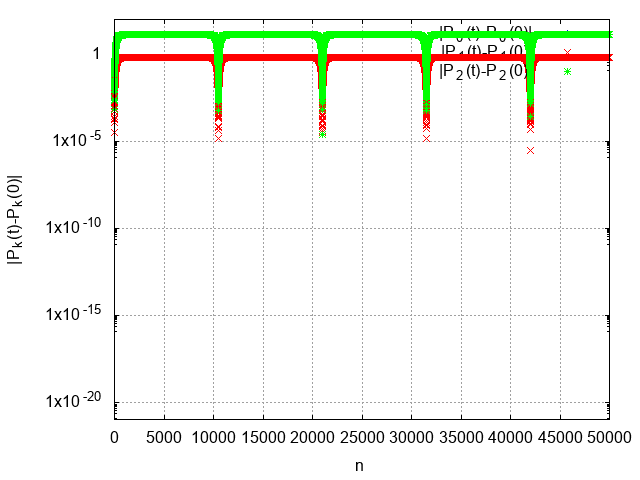
\includegraphics[scale=0.4]{{Korrekturen/plotting-Pk-P0-N2-}.png}
                \caption{Die Solitonwelle bewegt sich nach rechts und teilt sich entsprechend $ N=2 $ in zwei weitere Wellen auf. Im letzten Diagramm sieht man deutlich bei welchen Zeitpunkten sich die Wellen wieder vereinigen. Die Werte der Integrale sinken wieder auf Null runter. }                 
        \end{center}
\end{figure}
\newpage
Das selbe Phänomen können wir bei größeren Werten vom Parameter $ N $ feststellen.
Hier für 
\begin{align*}
        N = 3
\end{align*}
\begin{figure}[htp!]
        \begin{center}
                \includegraphics[scale=0.4]{{Korrekturen/korteweg_frame1-0-0.1-20.0-3.0-0.5-0.3}.png}  
                \includegraphics[scale=0.4]{{Korrekturen/korteweg_frame3200-0-0.1-20.0-3.0-0.5-0.3}.png}
                \includegraphics[scale=0.4]{{Korrekturen/korteweg_frame5400-0-0.1-20.0-3.0-0.5-0.3}.png}
                \includegraphics[scale=0.4]{{Korrekturen/korteweg_frame50000-0-0.1-20.0-3.0-0.5-0.3}.png}
                \includegraphics[scale=0.4]{{Korrekturen/plotting-Pk-P0-N3-}.png}
                \caption{Die Solitonwelle bewegt sich nach rechts und teilt sich entsprechend $ N=3 $ in drei weitere Wellen auf. Im letzten Diagramm sieht man deutlich bei welchen Zeitpunkten sich die Wellen wieder vereinigen. Die Werte der Integrale sinken wieder auf Null runter. }                 
        \end{center}
\end{figure}
Für den Fall $ N = 2,5 $ beobachten wir fasst das selbe, im Unterschied zu dem davor, haben wir hier eine kleinere Welle die sich sehr langsam bewegt und viele winzige Wellen, die sich nach links bewegen.
\begin{figure}[htp!]
        \begin{center}
                \includegraphics[scale=0.4]{{Korrekturen/korteweg_frame1-0-0.1-20.0-2.5-0.5-0.3}.png}  
                \includegraphics[scale=0.4]{{Korrekturen/korteweg_frame22400-0-0.1-20.0-2.5-0.5-0.3}.png}
                \includegraphics[scale=0.4]{{Korrekturen/korteweg_frame44000-0-0.1-20.0-2.5-0.5-0.3}.png}
                \includegraphics[scale=0.4]{{Korrekturen/korteweg_frame50000-0-0.1-20.0-2.5-0.5-0.3}.png}
                \includegraphics[scale=0.4]{{Korrekturen/plotting-Pk-P0-N2.5-}.png}
                \caption{Die Solitonwelle bewegt sich nach rechts und teilt sich entsprechend $ N=2,5 $ in drei weitere Wellen auf. Im letzten Diagramm sieht man deutlich bei welchen Zeitpunkten sich die Wellen wieder vereinigen. Die Werte der Integrale sinken wieder auf Null runter. }                 
        \end{center}
\end{figure}
\newpage
\subsection{Wassertiefenfunktion $ \nh_1 $}
In dieser neuen Betrachtung der Wassertiefe haben die folgenden Dinge verändert: Die Größe des Gitters $ G $ erhöht, die Länge $ L $ der Stufe im Wasser und dementsprechend die Simulationszeit erhöht. 
Für die erste Wassertiefenfunktion $ \nh_1 (x) $ von Gleichung \ref{eq:h1} benutzen wir für die Höhen $ h_0= 0,2\,, 0,3 $
\begin{align*}
\Delta \nx = 0,05\,, -8<G<40\,, N = 1\,, x_0=G\cdot 0,1 \;.
\end{align*}
Für größere Höhen benutzen wir
\begin{align*}
\Delta \nx = 0,1\,, -20<G<100\,, N = 1\,, x_0=G\cdot 0,1 \;.
\end{align*}
\begin{figure}[htp!]
        \begin{center}
                \includegraphics[scale=0.4]{{Korrekturen/korteweg_frame17000-1-0.05-8.0-1.0-0.2--0.1}.png}
                \includegraphics[scale=0.4]{{Korrekturen/korteweg_frame20000-1-0.05-8.0-1.0-0.3--0.1}.png}
                \includegraphics[scale=0.4]{{Korrekturen/korteweg_frame7000-1-0.1-20.0-1.0-0.4--0.1}.png}
                \includegraphics[scale=0.4]{{Korrekturen/korteweg_frame9000-1-0.1-20.0-1.0-0.5--0.1}.png}
                \includegraphics[scale=0.4]{{Korrekturen/korteweg_frame16000-1-0.1-20.0-1.0-0.6--0.1}.png}  
                \includegraphics[scale=0.4]{{Korrekturen/korteweg_frame16000-1-0.1-20.0-1.0-0.7--0.1}.png}
                \includegraphics[scale=0.4]{{Korrekturen/korteweg_frame16000-1-0.1-20.0-1.0-0.8--0.1}.png}
                \includegraphics[scale=0.4]{{Korrekturen/korteweg_frame24000-1-0.1-20.0-1.0-0.9--0.1}.png}
                \caption{Von links nach rechts von oben nach unten, sind die Abbildungen mit aufsteigender Höhe $ h_0 $ angeordnet. Es ist immer das Endprodukt der Simulation zu sehen. Die Solitonwelle bewegt sich nach rechts und transformiert sich an der Anhöhe in ein viel größere Welle. Die Amplitude steigt sehr schnell an. Die übrig gebliebene Wellenberg teilt sich weiter in kleinere Welle auf.}                 
        \end{center}
\end{figure}
\newpage
\subsubsection{Abhängigkeit der Amplitude $ \nA (h_0) $ von der Tiefe $ h_0 $} 
Dazu verwenden wir wieder die gleichen Parameter.
Die Schrittzahl wurde anhand der gewählten $ h_0 $ gesetzt.
\begin{figure}[htp!]
        \begin{center}
                \includegraphics[scale=0.7]{{plotting-A-h0-fit-1}.png}   
                \caption{Die Amplitude sinkt auf den Wert von $ A = 1 $ ab. Ein linearer Zusammenhang ist nur schwer zu vermuten.}
        \end{center}
\end{figure}
Für den linearen Fit erhalten wir
\begin{align}
\nA_1(h_0) = -25,23h_0 + 23,84 \label{eq:Ampk1}
\end{align}
Wenn wir die Werte für $ h_0 $ aus den Bereich  $ 0,1 < h_0 < 0,4 $ heraus nehmen und als Fit Funktion die Umkehrfunktion benutzen
\begin{align*}
        \nA_2(h_0) =  \frac{c}{h_0+e} + d
\end{align*}
bekommen wir
\begin{align}
\nA_2(h_0) =\frac{4,69}{h_0-0,17}-3,77\label{eq:Ampk2} \;.
\end{align}
\begin{figure}[htp!]
        \begin{center}
                \includegraphics[scale=0.7]{{plotting-A-h0-fit-2}.png}   
                \caption{Die Amplitudenfunktion $ \nA(h_0) $ ist eine Umkehrfunktion ohne die Werte von$ 0,1 < h_0 < 0,4 $. Vermutlich spielt hier die Wahl der Schrittweite $ \Delta \nx $ eine große Rolle. Für die Werte $ 0,1 < h_0 < 0,4 $ haben wir eine kleinere Schrittweite $ \Delta \nx = 0,05 $ benutzt.}
        \end{center}
\end{figure}
\newpage
\subsection{Wassertiefenfunktion $ \nh_2 $}
Für die zweite Wassertiefenfunktion $ \nh_2 $ von Gleichung \ref{eq:h2} nehmen wir die gleichen Veränderungen vor wie im vorherigen Abschnitt. Als Parameter wählen wir
\begin{align*}
\Delta \nx = 0,1\,, -30<G<90\,, N = 1\,, x_0=G\cdot -0,6\,, h_0=[0,3 , 0,4 , 0,5 , 0,6] \;.
\end{align*}
\begin{figure}[htp!]
        \begin{center}
                \includegraphics[scale=0.4]{{Korrekturen/korteweg_frame1-3-0.1-30.0-1.0-0.3--0.6}.png}
                \includegraphics[scale=0.4]{{Korrekturen/korteweg_frame10000-3-0.1-30.0-1.0-0.3--0.6}.png}
                \includegraphics[scale=0.4]{{Korrekturen/korteweg_frame30000-3-0.1-30.0-1.0-0.3--0.6}.png}\\
                \includegraphics[scale=0.4]{{Korrekturen/korteweg_frame1-3-0.1-30.0-1.0-0.4--0.6}.png}
                \includegraphics[scale=0.4]{{Korrekturen/korteweg_frame8400-3-0.1-30.0-1.0-0.4--0.6}.png}
                \includegraphics[scale=0.4]{{Korrekturen/korteweg_frame30000-3-0.1-30.0-1.0-0.4--0.6}.png}
                \caption{Von links nach rechts von oben nach unten, sind die Abbildungen mit aufsteigender Höhe $ h_0=[0,3 , 0,4] $ angeordnet Die Solitonwelle bewegt sich nach rechts und transformiert sich an der Anhöhe in ein viel größere Welle. Die Amplitude steigt sehr schnell an. Die übrig gebliebene Wellenberg teilt sich weiter in kleinere Welle auf. Die Amplitude nimmt mit steigender Höhe zu. Nach der Überquerung der Anhöhe geht die Solitonwelle fasst zurück zu ihrer Ursprungsgröße.}
        \end{center}
\end{figure}
\begin{figure}[htp!]
        \begin{center}
                \includegraphics[scale=0.4]{{Korrekturen/korteweg_frame1-3-0.1-30.0-1.0-0.5--0.6}.png}
                \includegraphics[scale=0.4]{{Korrekturen/korteweg_frame7200-3-0.1-30.0-1.0-0.5--0.6}.png}
                \includegraphics[scale=0.4]{{Korrekturen/korteweg_frame30000-3-0.1-30.0-1.0-0.5--0.6}.png}\\
                \includegraphics[scale=0.4]{{Korrekturen/korteweg_frame1-3-0.1-30.0-1.0-0.6--0.6}.png}
                \includegraphics[scale=0.4]{{Korrekturen/korteweg_frame6600-3-0.1-30.0-1.0-0.6--0.6}.png}
                \includegraphics[scale=0.4]{{Korrekturen/korteweg_frame30000-3-0.1-30.0-1.0-0.6--0.6}.png}
                \caption{Von links nach rechts von oben nach unten, sind die Abbildungen mit aufsteigender Höhe $ h_0=[ 0,5 , 0,6] $ angeordnet Die Solitonwelle bewegt sich nach rechts und transformiert sich an der Anhöhe in ein viel größere Welle.}                 
        \end{center}
\end{figure}


\newpage

\section{Programm}
Das Programm wurde in der Programmiersprache Julia(\url{https://julialang.org/}) geschrieben. 
Auf den nachfolgenden Seiten können sie den gesamten Code einsehen. 
Zusätzlich ist die gesamte Arbeit mit der Software noweb geschrieben worden.
In noweb kann alles in einer Datei gespeichert werden und in Latex die einzelnen Codeabschnitte übersichtlich dargestellt werden.
Das Programm kann mit Hilfe des Befehls

\begin{verbatim}
        julia korteweg.jl 0 5000 0.1 5.5 1 0.5 1 0.3 > filled.log
\end{verbatim}

gestartet werden. 
Dabei wird die gesamte Ausgabe in die Datei filled.log geschrieben.
Die Plots wurden mit gnuplot erstellt.
Die Parameter können direkt über eingeben werden über die Kommandozeile:
\begin{verbatim}
        julia korteweg.jl p1 p2 p3 p4 p5 p6 p7 p8
\end{verbatim}

mit

\begin{itemize}
        \item p1 - Variable \verb|schalter| 
        \item p2 - Variable \verb|n|, Ende der Schleife über $ n $
        \item p3 - Variable \verb|delta_x|
        \item p4 - Variable \verb|grenze|, Größe des Gitters $ G $
        \item p5 - Variable \verb|N|, Variable $ N $
        \item p6 - Variable \verb|h0|, Tiefe des Wassers $ h_0 $
        \item p7 - Schalter für Dateioutput ja oder nein
        \item p8 - Startposition $ x_0 $
\end{itemize}



\nwenddocs{}\nwbegindocs{2}\nwdocspar
\nwenddocs{}\nwbegincode{3}\sublabel{NW11YXi6-6Xpzo-1}\nwmargintag{{\nwtagstyle{}\subpageref{NW11YXi6-6Xpzo-1}}}\moddef{korteweg.jl~{\nwtagstyle{}\subpageref{NW11YXi6-6Xpzo-1}}}\endmoddef\nwstartdeflinemarkup\nwenddeflinemarkup
#= 
Korteweg de Vries Simulationsprogramm
=#
\LA{}PeriodicCond~{\nwtagstyle{}\subpageref{NW11YXi6-3SJnRd-1}}\RA{}
\LA{}Maximum~{\nwtagstyle{}\subpageref{NW11YXi6-ojQ28-1}}\RA{}
\LA{}Init~{\nwtagstyle{}\subpageref{NW11YXi6-13rLI-1}}\RA{}
\LA{}h Funktion~{\nwtagstyle{}\subpageref{NW11YXi6-3d19fz-1}}\RA{}
\LA{}NumCalc~{\nwtagstyle{}\subpageref{NW11YXi6-3QhXhc-1}}\RA{}
\LA{}IntCon~{\nwtagstyle{}\subpageref{NW11YXi6-2wD8Oc-1}}\RA{}
\LA{}Output~{\nwtagstyle{}\subpageref{NW11YXi6-2r7wy0-1}}\RA{}
\LA{}Main~{\nwtagstyle{}\subpageref{NW11YXi6-1uPnon-1}}\RA{}
\nwnotused{korteweg.jl}\nwendcode{}\nwbegindocs{4}\nwdocspar
\nwenddocs{}\nwbegincode{5}\sublabel{NW11YXi6-3SJnRd-1}\nwmargintag{{\nwtagstyle{}\subpageref{NW11YXi6-3SJnRd-1}}}\moddef{PeriodicCond~{\nwtagstyle{}\subpageref{NW11YXi6-3SJnRd-1}}}\endmoddef\nwstartdeflinemarkup\nwusesondefline{\\{NW11YXi6-6Xpzo-1}}\nwenddeflinemarkup
function PeriodicCond(pos)# Periodische Randbedingungen
  temp1 = u[pos,scal-3]
  temp2 = u[pos,scal-2]
  u[pos,1], u[pos,2],u[pos,scal-1], u[pos,scal] =
  temp1, temp2, u[pos,3], u[pos,4]
end
\nwused{\\{NW11YXi6-6Xpzo-1}}\nwendcode{}\nwbegindocs{6}\nwdocspar
\nwenddocs{}\nwbegincode{7}\sublabel{NW11YXi6-ojQ28-1}\nwmargintag{{\nwtagstyle{}\subpageref{NW11YXi6-ojQ28-1}}}\moddef{Maximum~{\nwtagstyle{}\subpageref{NW11YXi6-ojQ28-1}}}\endmoddef\nwstartdeflinemarkup\nwusesondefline{\\{NW11YXi6-6Xpzo-1}}\nwenddeflinemarkup
function Maximum(n)
  max = 0
  if n == 1
    for i in 3:(scal-2)
      if max < u[1,i]
        max = u[1,i]
      end
    end
  else
    for i in 3:(scal-2)
      if max < u[3,i]
        max = u[3,i]
      end
    end
  end
  return max
end
\nwused{\\{NW11YXi6-6Xpzo-1}}\nwendcode{}\nwbegindocs{8}\nwdocspar
\nwenddocs{}\nwbegincode{9}\sublabel{NW11YXi6-13rLI-1}\nwmargintag{{\nwtagstyle{}\subpageref{NW11YXi6-13rLI-1}}}\moddef{Init~{\nwtagstyle{}\subpageref{NW11YXi6-13rLI-1}}}\endmoddef\nwstartdeflinemarkup\nwusesondefline{\\{NW11YXi6-6Xpzo-1}}\nwenddeflinemarkup
function Init()
  global file = open("P_K-data.txt","w")
  global P0alt =0.
  global P1alt =0.
  global P2alt =0.
  global printer =Int64[0:200:parse(Int64,ARGS[2]);]# Variable zur Steuerung der 
  #Ausgabe von Dateien, alle 200 Schritt erfolgt die Ausgabe
  printer[1]=1
  global schalter=parse(Int,ARGS[1])
  global N = parse(Float64,ARGS[5]) # N- Soliton Lösung
  global delta_x = parse(Float64,ARGS[3])
  global delta_t = 2*delta_x/(3*sqrt(3)*(-2*(N*(N+1))+1/(delta_x)^2))*0.7
  global grenze = parse(Float64,ARGS[4]) # Größe des Gitters
  global L = grenze*0.3
  global h0 = parse(Float64,ARGS[6]) # Tiefe des Wassers
  global l = Int64(2)
  global pil = Int(1)
  global x = Float64[-grenze:delta_x:3*grenze;] # x Koordinate
  global scal = length(x)+4# Indexgröße von u festlegen
  global u = (zeros(Float64,3,scal)) # dimensionslose Anhebung
  for i in 3:(scal-2) #Anfangsbedinung anlegen
    u[1,i] = ((N*(N+1))/(cosh(x[i-2]+grenze*(-parse(Float64,ARGS[8]))))^2)
  end
  println("reset")
  println("#$(parse(Int,ARGS[1]))-$(parse(Float64,ARGS[2]))-\\\\
  $(parse(Float64,ARGS[3]))-$(parse(Float64,ARGS[4]))-\\\\
  $(parse(Float64,ARGS[5]))-$(parse(Float64,ARGS[6]))-\\\\
  $(parse(Float64,ARGS[7]))-$(parse(Float64,ARGS[8]))")
  println("# Maxmimum $(Maximum(1))")
  println("set grid")
  println("set xrange [",-grenze,":",3*grenze,"]")
  println("set yrange [",-2,":",N*(N+5)/h0,"]")#4.5 , 10.5 , 18
  println("set xlabel 'x'")
  println("set ylabel 'u'")
end
\nwused{\\{NW11YXi6-6Xpzo-1}}\nwendcode{}\nwbegindocs{10}\nwdocspar
\nwenddocs{}\nwbegincode{11}\sublabel{NW11YXi6-3d19fz-1}\nwmargintag{{\nwtagstyle{}\subpageref{NW11YXi6-3d19fz-1}}}\moddef{h Funktion~{\nwtagstyle{}\subpageref{NW11YXi6-3d19fz-1}}}\endmoddef\nwstartdeflinemarkup\nwusesondefline{\\{NW11YXi6-6Xpzo-1}}\nwenddeflinemarkup
function h(pos)
  if (schalter == 1) # h_1(x) Funktion
    if (x[pos] < 0)
      return 1
    elseif (0<=x[pos])&&(x[pos]<=L)
      return 1/2*(1+h0+(1-h0)*cos(pi*(x[pos])/L))
    else
      return h0
    end
  elseif (schalter == 2) # eine Testfunktion
    if (L<=x[pos])&&(x[pos]<=2*L)
      return 1/2*(1+h0+(1-h0)*cos(pi*(x[pos]+L)/L))
    elseif x[pos] > L
      return h0
    elseif (x[pos]<=-grenze+L)&&(x[pos]>=-grenze)
      return 1/2*(1+h0+(1-h0)*cos(pi*(x[pos]-grenze+L)/L))
    else
      return 1
    end
  elseif (schalter == 3) # h_2(x) Funktion
    return  (1-h0*exp(-x[pos]*x[pos]/(L*L)))
  else
    return 1
  end
end
\nwused{\\{NW11YXi6-6Xpzo-1}}\nwendcode{}\nwbegindocs{12}\nwdocspar
\nwenddocs{}\nwbegincode{13}\sublabel{NW11YXi6-3QhXhc-1}\nwmargintag{{\nwtagstyle{}\subpageref{NW11YXi6-3QhXhc-1}}}\moddef{NumCalc~{\nwtagstyle{}\subpageref{NW11YXi6-3QhXhc-1}}}\endmoddef\nwstartdeflinemarkup\nwusesondefline{\\{NW11YXi6-6Xpzo-1}}\nwenddeflinemarkup
function NumCalc(n)
   for i in 3:(scal-2) # Zabuski-Kruskal Schema
      if n == 2
         u[2,i]=u[1,i] - delta_t*(((h(i-2))^(-7/4))*
         (u[1,i-1]+u[1,i]+u[1,i+1])*
         (u[1,i+1]-u[1,i-1])/delta_x+(h(i-2)^(1/2))*
         (u[1,i+2]-2*u[1,i+1]+2*u[1,i-1]-u[1,i-2])/
         (2*(delta_x)^3))
         global l=2
      else
         u[3,i]=u[1,i] - 2*delta_t*(((h(i-2))^(-7/4))*
         (u[2,i-1]+u[2,i]+u[2,i+1])*
         (u[2,i+1]-u[2,i-1])/delta_x+(h(i-2)^(1/2))*
         (u[2,i+2]-2*u[2,i+1]+2*u[2,i-1]-u[2,i-2])/
         (2*(delta_x)^3))
         global l=3
      end
   end
end
\nwused{\\{NW11YXi6-6Xpzo-1}}\nwendcode{}\nwbegindocs{14}\nwdocspar
\nwenddocs{}\nwbegincode{15}\sublabel{NW11YXi6-2wD8Oc-1}\nwmargintag{{\nwtagstyle{}\subpageref{NW11YXi6-2wD8Oc-1}}}\moddef{IntCon~{\nwtagstyle{}\subpageref{NW11YXi6-2wD8Oc-1}}}\endmoddef\nwstartdeflinemarkup\nwusesondefline{\\{NW11YXi6-6Xpzo-1}}\nwenddeflinemarkup
function IntCon(pos,n)
  P0=Float64(0)
  for i in 3:(scal-2)
    P0=P0+(1/3*(u[pos,i-1]+u[pos,i]+u[pos,i+1]))*delta_x
  end
  P1=Float64(0)
  for i in 3:(scal-2)
    P1=P1+((1/3*(u[pos,i-1]+u[pos,i]+u[pos,i+1]))^2)*delta_x
  end
  P2=Float64(0)
  for i in 3:(scal-2)
    P2=P2+(2*(1/3*(u[pos,i-1]+u[pos,i]+u[pos,i+1]))^3-
      ((u[pos,i+1]-u[pos,i-1])/delta_x/2)^2)*delta_x
  end
  #println("set label 3 \\"P0= ",
  # trunc(P0,digits=10)," \\" at screen 0.6,0.8")# Anzeige des Integrals im Diagramm
  #println("set label 2 \\"P1= ",
  # trunc(P1,digits=10)," \\" at screen 0.6,0.75")# Anzeige des Integrals im Diagramm
  #println("set label 1 \\"P2= ",
  # trunc(P2,digits=10)," \\" at screen 0.6,0.7")# Anzeige des Integrals im Diagramm
  if n>1
    #write(file,"$n $(trunc(abs(Pk[1]-P0),digits=10)) $(trunc(abs(Pk[2]-P1),digits=10)) $(trunc(abs(Pk[3]-P2),digits=10)) \\n")
    write(file,"$n $(abs(Pk[1]-P0)) $(abs(Pk[2]-P1)) $(abs(Pk[3]-P2)) \\n")
    #write(file,"$n $(abs(Pk[1]-P0)) $(Pk[1]) \\n")
  else
    global Pk=zeros(3)
    Pk[1]=P0
    Pk[2]=P1
    Pk[3]=P2
    write(file,"$n 0 0 0 \\n")
    #write(file,"$n $(Pk[1]) $(Pk[2]) $(Pk[3]) \\n")
  end
end
\nwused{\\{NW11YXi6-6Xpzo-1}}\nwendcode{}\nwbegindocs{16}\nwdocspar
\nwenddocs{}\nwbegincode{17}\sublabel{NW11YXi6-2r7wy0-1}\nwmargintag{{\nwtagstyle{}\subpageref{NW11YXi6-2r7wy0-1}}}\moddef{Output~{\nwtagstyle{}\subpageref{NW11YXi6-2r7wy0-1}}}\endmoddef\nwstartdeflinemarkup\nwusesondefline{\\{NW11YXi6-6Xpzo-1}}\nwenddeflinemarkup
function Output(pos, tsim, treal, n) # Ausgabe ins Terminal
  if (pil <= length(printer)) & ( parse(Int,ARGS[7])> 0 )
    if (n == printer[pil]) 
      #println("set term qt;")
      println("set term png; set output sprintf('korteweg_frame$n-$(parse(Int,ARGS[1]))-$(parse(Float64,ARGS[3]))-$(parse(Float64,ARGS[4]))-$(parse(Float64,ARGS[5]))-$(parse(Float64,ARGS[6]))-$(parse(Float64,ARGS[8])).png');")
      global pil = pil+1
      println("set label 5 \\"sim time= ",
      trunc(tsim,digits=10)," \\" at screen 0.6,0.9")# Anzeige der Zeit im Diagramm
      println("set label 6 \\"n= ",n," \\" at screen 0.6,0.85")
      if (schalter == 1) # Anzeige der h_1,2 Funktionen im Diagramm
      println("plot '-' w l, [-$grenze:0] -1 linecolor 3 notitle, [0:$L] \\\\
      -(1+$(h0)+(1-$(h0))*cos(pi*x/$(L)))/2 linecolor 3 notitle, \\\\
      [$L:$(5*grenze)] -$(h0) linecolor 3 notitle")
      elseif (schalter == 2)
        println("plot '-' w l, [$L:$(2*L)] (1+$(h0)+(1-$(h0))*cos((pi*(x+$L))/$L))/2-1\\\\
        linecolor 3 notitle, [-$(grenze):$(-grenze+L)] (1+$(h0)+\\\\
        (1-$(h0))*cos(pi*(x-$(grenze+L))/$L))/2-1 linecolor 3 notitle, \\\\
        [$(-grenze+L):$L] 1-1 linecolor 3 notitle, [$(2*L):$grenze] $(h0)-1 linecolor 3 notitle") 
      elseif (schalter == 3)
        println("plot '-' w l, [-$grenze:$(3*grenze)] -(1-$(h0)*exp(-x*x/$(L*L))) linecolor 3 notitle")
      else
        println("plot '-' w l")
      end
      global y=zeros(scal-4)
      for i in 3:(scal-2) # Werteausgabe 
        println(x[i-2]," ",u[pos,i])
      end
      println("elapsed time: 0.672879991 seconds")
    end
  end
  if n == (parse(Int,ARGS[2])) # Maximum Anzeige und Berechnung
    println("# Maxmimum $(Maximum(n))")
  end
  #close("P_K.txt")
end
\nwused{\\{NW11YXi6-6Xpzo-1}}\nwendcode{}\nwbegindocs{18}\nwdocspar
\nwenddocs{}\nwbegincode{19}\sublabel{NW11YXi6-1uPnon-1}\nwmargintag{{\nwtagstyle{}\subpageref{NW11YXi6-1uPnon-1}}}\moddef{Main~{\nwtagstyle{}\subpageref{NW11YXi6-1uPnon-1}}}\endmoddef\nwstartdeflinemarkup\nwusesondefline{\\{NW11YXi6-6Xpzo-1}}\nwenddeflinemarkup
for n in 1:(parse(Int,ARGS[2]))
   if n == 1
      global treal=0.
      global tsim=0.
      Init()
      IntCon(n,n)
      PeriodicCond(n)
      tsim=delta_t
      Output(n, tsim, treal, n)
   else
      NumCalc(n)
      PeriodicCond(l)
      if n>2 #Vertauschung der Reihen in dem Array der Anhebung
         for k in 1:scal
            temp3=u[2,k]
            u[2,k]=u[3,k]
            u[1,k]=temp3
         end
      end
      tsim=tsim+delta_t
      #println("elapsed time: 0.672879991 seconds")
      IntCon(l,n)
      Output(l, tsim, treal, n)
   end
end

\nwused{\\{NW11YXi6-6Xpzo-1}}\nwendcode{}\nwbegindocs{20}\nwdocspar
\begin{comment}

\nwenddocs{}\nwbegindocs{21}\nwdocspar
@language python
from subprocess import call
#
##### Meta
'''
Programmiersprache: julia
Methoden:
    - Vertauschung von Zeilen einer (3)x(n) Matrix
    - Kommandozeilenargumente fürs Julia Programm nutzen
    - gnuplot live plot, die Daten werden sofort live angezeigt über shell pipes
    - 1. Verwendung von noweb
    - 1. Verwendung von Leo Editor als Programmierumgebung
    - Punkte im Dateiname in Latex (Quelle: https://tex.stackexchange.com/questions/10574/includegraphics-dots-in-filename)
    - PyPlot Benutzung bei Script in der Kommandozeile den Paramter -i setzen
    - 1. Verwendung von Ausgabe in Julia in Dateien, nicht nur über die Kommandozeile
'''
'''
Korrekturaufgaben vom Hernn Pikovski
  + Zeigen Sie analytisch, dass (6) gilt (berechnen Sie die Zeitableitungen in (6), setzen Sie die KdV-Gleichung und zeigen, dass (6) gilt)
  + Auch numerisch - zeigen Sie |P_k(t)-P_k(0)| aus Ihren Rechnungen in logarithmischen Skala 
    + Programmierung
    + Protokoll
  + Fuehren Sie die Simulationen im Abschnitt 3 fuer laengeren Zeit, auf einem groesserem Interval (um zB zu sehen, was mit der "Restwellen" fuer N=2,5 passiert)
    + Plot der Simulation
    + Plot der Momente
    + Protokoll
  + Im Abschnitt 4: waehlen Sie bitte L etwas groesser (groesser als die Soliton-Laenge), dabei koennen Sie die Stufe nicht in der mitte, sondern etwas links plazieren. Zeigen Sie Bilder wie Abb 3 fuer verschiedene h_0. Aehnlich fuer Abb 6 - dort soll der Bereich groesser sein, um zu sehen, on ein Soliton nach dem Huegel sich formiert.
    + Plot der Simulation für verschiedene h_0
    + Protokoll
                
Korrekturaufgaben vom Hernn Pikovski Teil 2
  +(1 Zum 6.1 : Erhaltung der Momente soll nicht fuer die Soliton-Loesung gezeigt werden, sondern fuer eine allgemeine Loesung mit (beliebigen) Anfangsbedingungen im begrenzten Bereich (so dass im Unendlichen das Feld verschwindet)
    +Protokoll  
  +(2 Abb 7-9: wie gross ist \Delta t ?
    +Protokoll
  +(3 Abb 7-9: zeichnen Sie die Integralen-Abweichungen |P_k(t)-P_k(0)| mit der logarithmishen Skala, also log|P_k(t)-P_k(0)| vs Zeit
    +gnuplot - Dias
    +Protokoll
  +(4 Geben Sie die Formeln, mit welchen die Integrale berechnet sind
    +Protokoll
  +(5 Anhand der Abb. 10 machen Sie bitte die Abb. 4-5 neu
    +Rechnung
    +Protokoll
  +(6 Abb 11: koennten Sie bitte weiter rechnen, so dass man sieht was passiert nachdem der Soliton ueber die Schwelle ist
    +Protokoll
'''
##### Historie
'''
20.2.2019
   - Testatgespräch mit Herrn Pikoski
      - Kritikpunkte:
         - keine genaue Angabe der Genauigkeit
         - Variable genau definieren mit welchen Typ sie initialisiert werden
         - das erste Integral ist dann auch nicht genau Null sondern sehr sehr klein im Vergleich zu den anderen beiden Integralen
   - Überprüfung der Genauigkeit der Integrale über genaue Variabledefinition mit Float64
   - Variablendefinition von allen float Variablen vorgenommen zu Float64
   
19.2.2019
   - Abschluss der letzten Korrekturen am Protokoll
13.2.2019
    - Teil 2 der Korrekturen beendet
4.2-7.2.2019
    - Korrekturen Pikovskis ins Programm und Protokoll eingepflegt Details siehe Abschnitt 'Korrekturen' hier und im Protokoll
10.1.2019
    - Fertigstellung des Protokolls
        
8.1.2019
    - Die letzte Aufgabe gelöst und muss nur noch ins Protokoll geschrieben werden
    - Im Programm die h(x) Funktion genau implmentiert und geplottet
    - Amplitude-h0 Plot fertig gestellt
    - die verwendeten Daten sind in der Daten-h0.txt Datei
5.1.2019
    - Programm bereinigt, alles funktioniert wieder
3.8.2018
    - Plotmethode geändert: zuerst Datei mit Daten füllen, dann gnuplot die Datei auswerten lassen
    - Fertigstellung der Plotausgabe über PyPlot
3.6.2018
    - Die Berechnung der Integrale überprüft und neu geschrieben. 
    - Aufgabe 1 vollständig protokolliert.
    - Idee: vielleicht 3d Modell bauen mit t,x,u Achsen
    - todo.cp2: Aufgabe 2 Diagramme vorbereiten und nochmal Aufgaben klären
30.5.2018
    - Lösung für Punkte im Dateinamen in Latex \includegraphics{{bild0.1-0.1}.png}
    - Lösung für die Anzeige der Nachkommastelle mittels trunc(Zahl, Nachkommastelle) Funktion
26.5.2018 
    - Bilder für die 1. Aufgabe erzeugt. Die Bilder befinden sich in dem Unterordner Aufgabe 1. 
17.5.2018 
    - Bilder werden von der laufenden Simulation in 200 Schritten abgespeichert, nebenbei läuft die Anzeige des Diagramms weiter
16.5.2018
    - T Kapitel Korteweg-de-Vries Gleichung, Numerisches Lösungsverfahren: ..., und Korteweg-de-Vries Gleichung bei variabler Tiefe geschrieben
    - todo.cp2: Überlegung ob Quellcode gleich mit einbeziehen
    - done.cp2: Bilder der Simluation für die Problemstellungen erzeugen, dazu ein bisschen Programmierarbeit nötig
20.4.2018 
    - Anfang der Einleitung
16.4.2018 
    - Bei der Compilation einen neuen Parameter gesetzt, der die Variable h0 steuert
    - ein paar Kommentare im Code gesetzt
    - die Compilation stabiler gemacht durch hinzufügen eines '&' Symbols am Ende jedes Kommandos 
    - Tests für die Abhängigkeit der Amplitude von h0 gemacht
    - offen was genau gezeigt, geplottet werden soll mit N(h0) bzw. N*(N+1) abh. h0
9.4.2018 
    - die Variable schalter erweitert 
    - die h(x) Funktion erweitert mit der exp() Funktion
    - gelungener Testlauf mit der neuen h(x) Funktion
    - überprüft ob alle Aufgaben erfüllt sind: offen: Amplitudenabhängigkeit ermitteln
    - Doku: Parameterübergabe an das julia Programm wo welcher Parameter übergeben wird beim Programm aufruf
4.4.2018
    - Umstrukturierung der noweb Datei: Einfügung des Leo Buttons
    - Erweiterung der Shell Argumente fürs julia Script 
    - Historie.log ist jetzt in der noweb Datei
    - Erweiterung des Outputs: gnuplot output in png möglich
    - Komprimierung der Dateien ausgestellt
    - Versions.conf ist jetzt Teil der noweb der Datei
28.3.2018
    - Einpflegung ins Leo Programm über die CodeFabrik.leo Datei.
    - Shell Argumente fürs julia Script eingefügt.
15.1.2018
    - Programm funktioniert wieder mit Einrückung und einen Schalter zum umschalten zwischen Problem 1 und Problem 2
'''


##### Dokumentation
## Methode zum Erzeugen des Julia Quellcodes
g.execute_shell_commands("echo '----------------Start ----------------'")
#print('start')
g.execute_shell_commands("notangle -Rkorteweg.jl korteweg-de-vries.nw > korteweg.jl")

## Methode zur Erzeugung von html Seiten

#g.execute_shell_commands("noweave -filter l2h -index -autodefs c -html korteweg-de-vries.nw > korteweg-de-vries.html &")


##### Debug

#g.execute_shell_commands("julia korteweg.jl 0 3 0.1 2.4 2 0.5 0 &")
#g.execute_shell_commands("julia korteweg.jl 0 3 0.1 2.4 2 0.5 0 | gnuplot -p &")

##### Compilation ohne Leo Editor
'''
g.execute_shell_commands("notangle -Rkorteweg.jl korteweg-de-vries.nw | julia | gnuplot -p &")

g.execute_shell_commands("notangle -Rkorteweg.jl korteweg-de-vries.nw > korteweg.jl && julia korteweg.jl 1 500000 | gnuplot -p &")

'''
##### Projekt PyPlot ohne Gnuplot plotten

#g.execute_shell_commands("julia -i korteweg.jl 0 5000 0.1 5.5 3 0.5 0 &")

## Parameterübergabeerklärung
'''
julia korteweg.jl p1 p2 p3 p4 p5 p6 p7 p8 

p1 - Variable schalter 
p2 - Ende der Schleife über n
p3 - Variable delta_x
p4 - Variable grenze, Größe des Gitters
p5 - Variable N
p6 - Variable h0, Tiefe des Wassers
p7 - Schalter für Dateioutput ja oder nein
p8 - Startposition
'''

##### Aufgabe 1

## TODO Herleitung des Stabilitätskriteriums

## N = 1

#g.execute_shell_commands("julia korteweg.jl 0 5000 0.1 5.5 1 0.5 1 0.3 | gnuplot -p &")
g.execute_shell_commands("time julia korteweg.jl 0 8000 0.1 10.5 3 0.5 1 0.3 > filled.log")

## N = 2
# sind folgende Parameter nötig delta_x = 0.1 grenze = 4.4

#g.execute_shell_commands("julia korteweg.jl 0 5000 0.1 5.5 2 0.5 1 0.3 | gnuplot -p &")
#g.execute_shell_commands("time julia korteweg.jl 0 50000 0.1 20 2 0.5 1 0.3 > filled.log")
#g.execute_shell_commands("time julia korteweg.jl 0 500 0.1 20 2 0.5 0 0.3 > filled.log")

## N = 2,5
#g.execute_shell_commands("julia korteweg.jl 0 5000 0.1 5.5 2.5 0.5 1 0.3 | gnuplot -p &")
#g.execute_shell_commands("julia korteweg.jl 0 50000 0.1 20 2.5 0.5 1 0.3 > filled.log")

## N = 3, delta_x=0.05 grenze = 5.4 ohne sleep
# bis einschließlich N = 5 reicht delta_x=0.05 und grenze = 5.4 vollkommen aus

#g.execute_shell_commands("julia korteweg.jl 0 5000 0.1 5.5 3 0.5 1 0.3 | gnuplot -p &")
#g.execute_shell_commands("time julia korteweg.jl 0 50000 0.1 20 3 0.5 1 0.3 > filled.log")

## Tests mit N als rationale Zahl, zum Teil sehr krummen Zahlen
#g.execute_shell_commands("julia korteweg.jl 0 5000 0.05 10.5 4.644674 0.5 0 0.3 | gnuplot -p &")
#g.execute_shell_commands("julia korteweg.jl 0 5000 0.05 10.5 6.644674 0.5 0 0.3 > filled.log")

##### Aufgabe 2

##Profilfunktion 1 also die originale h(x) Funktion
#g.execute_shell_commands("time julia korteweg.jl 1 9000 0.1 20 1 0.4 1 -0.2 > filled.log")


##Beschreibung für den Plot von Amplitude zur Höhe h_0
#g.execute_shell_commands("time julia korteweg.jl 1 26000 0.05 16.4 1 0.1 0 -0.2 > filled-0.1---.log")
#bei 0.1 muss man 0.05 als Schrittweite verwenden sonst explodiert die Lösung




## Profilfunktion 2 dabei den schalter auf 2 setzen
# funktioniert mit diesen Paramtern 2 500000 0.05 4.4 2 0.5 0

#g.execute_shell_commands("julia korteweg.jl 2 6000 0.05 7.5 1 0.3 0 0 > filled.log")
#g.execute_shell_commands("julia korteweg.jl 2 40000 0.05 5.5 1 0.5 0 0.3 > filled.log")

## Profilfunktion 3 mit exp(.) dabei den schalter auf 3 setzen

#g.execute_shell_commands("julia korteweg.jl 3 5000 0.05 10.4 1 0.8 0 0.5 | gnuplot -p &")
#g.execute_shell_commands("julia korteweg.jl 3 20000 0.05 10.4 1 0.5 1 0 > filled.log")
#g.execute_shell_commands("julia korteweg.jl 3 40000 0.05 10.4 1 0.5 1 -0.4 > filled.log")


# erster Test ergab bei sim time = 1.0 ein großes Soliton, für n=500000,delta_x=0.05 ,größe=10.4,N=3, h0=0.5 funktioniert
# Bei N = 3 geht es von 0 bis 0.7, dann explodiert die Lösung
# ??? # 




##### testing

#g.execute_shell_commands("julia korteweg.jl 2 6000 0.025 5.5 2 0.5 0 > filled.log")

####Korrekturen
# h0 Simulation mit rechte Grenze neu mit 5*grenze und grenze = 20
#g.execute_shell_commands("time julia korteweg.jl 1 7000 0.05 20 1 0.3 1 -0.1 > filled.log")


#h0 für die exponentielle Funktion verändern
#g.execute_shell_commands("time julia korteweg.jl 3 30000 0.1 30 1 0.6 1 -0.6 > filled.log")

'''
welche Bilder für die Korrekturen werden benutzt bzw sind die richtigen
korteweg_frame17000-1-0.05-8.0-1.0-0.2--0.1.png -0.2
korteweg_frame20000-1-0.05-8.0-1.0-0.3--0.1.png -0.3
korteweg_frame7000-1-0.1-20.0-1.0-0.4--0.1.png -0.4
korteweg_frame9000-1-0.1-20.0-1.0-0.5--0.1.png -0.5
korteweg_frame16000-1-0.1-20.0-1.0-0.6--0.1.png -0.6
korteweg_frame16000-1-0.1-20.0-1.0-0.7--0.1.png -0.7
korteweg_frame16000-1-0.1-20.0-1.0-0.8--0.1.png -0.8
korteweg_frame24000-1-0.1-20.0-1.0-0.9--0.1.png -0.9


korteweg_frame7000-1-0.1-20.0-1.0-0.4--0.1.png -0.4
korteweg_frame9000-1-0.1-20.0-1.0-0.5--0.1.png -0.5
korteweg_frame24000-1-0.1-20.0-1.0-0.9--0.1.png -0.9
korteweg_frame8800-1-0.1-20.0-1.0-0.9--0.1.png
korteweg_frame16000-1-0.1-20.0-1.0-0.8--0.1.png -0.8
korteweg_frame7600-1-0.1-20.0-1.0-0.8--0.1.png
korteweg_frame16000-1-0.1-20.0-1.0-0.7--0.1.png -0.7
korteweg_frame16000-1-0.1-20.0-1.0-0.6--0.1.png -0.6
korteweg_frame17000-1-0.05-8.0-1.0-0.2--0.1.png -0.2
korteweg_frame20000-1-0.05-8.0-1.0-0.3--0.1.png -0.3
korteweg_frame11000-1-0.1-20.0-1.0-0.6--0.2.png
korteweg_frame9000-1-0.1-20.0-1.0-0.4--0.2.png
korteweg_frame10000-1-0.1-20.0-1.0-0.5--0.2.png
'''
####
g.execute_shell_commands("echo '----------------Gnuplot Start----------------'")
g.execute_shell_commands("gnuplot filled.log -p &")
g.execute_shell_commands("echo '----------------Gnuplot Ende ----------------'")

\nwenddocs{}\nwbegindocs{22}\nwdocspar
@language python
##### Programm zum Start der Versionisierung des Codes
from subprocess import call
g.execute_shell_commands("notangle -RVersions.conf korteweg-de-vries.nw > Versions.conf &")
g.execute_shell_commands("/home/christian/Programme/storeBackup/bin/storeBackup.pl -f Versions.conf &")

\nwenddocs{}\nwbegindocs{23}\nwdocspar

@language python
##### Programm zum Start der Versionisierung des Codes
from subprocess import call

##Methode zur Erzeugung der Plotdatei für die Amplitude
g.execute_shell_commands("notangle -Rploth0.plt korteweg-de-vries.nw > ploth0.plt")

g.execute_shell_commands("gnuplot ploth0.plt -p &")

## Werte für die Fitfunktionen
#a = 3.40825     
#b= 3.04851  
#c = -5.44657     
#d = 7.52866

\nwenddocs{}\nwbegindocs{24}\nwdocspar

@language python
##### Programm zum Start der Versionisierung des Codes
from subprocess import call

##Methode zur Erzeugung der Plotdatei für die Amplitude
g.execute_shell_commands("notangle -RplotPk-P0.plt korteweg-de-vries.nw > plotPk-P0.plt")

g.execute_shell_commands("gnuplot plotPk-P0.plt -p &")

## Werte für die Fitfunktionen
#a = 3.40825     
#b= 3.04851  
#c = -5.44657     
#d = 7.52866

\nwenddocs{}\nwbegindocs{25}\nwdocspar

\nwenddocs{}\nwbegincode{26}\sublabel{NW11YXi6-3JYCji-1}\nwmargintag{{\nwtagstyle{}\subpageref{NW11YXi6-3JYCji-1}}}\moddef{ploth0.plt~{\nwtagstyle{}\subpageref{NW11YXi6-3JYCji-1}}}\endmoddef\nwstartdeflinemarkup\nwenddeflinemarkup
reset
set grid
set yrange [0:20]
set ylabel 'A'
set term png
###
set xrange [0:1.2]
set xlabel 'h_0'
set output sprintf('plotting-A-h0-.png')
plot "h0-daten.txt" using ($1):($4) title 'Amplitude A(h_0)' lt rgb 'blue'
A_1(x) = a*x + b
A_2(x) = c/(x+e)+ d
fit [0:0.9] [0:20] A_1(x) 'h0-daten.txt' using ($1):($5) via a,b
fit [0.4:1] [0:20] A_2(x) 'h0-daten.txt' using ($1):($5) via c,d,e#
set output sprintf('plotting-A-h0-fit-1.png')
plot "h0-daten.txt" using ($1):($5) title 'Amplitude A(h_0)' lt rgb 'blue', A_1(x) lt rgb 'red'#, A_2(x) lt rgb 'brown'
set output sprintf('plotting-A-h0-fit-2.png')
plot [0.3:1.2][0:20] "h0-daten.txt" using ($1):($5) title 'Amplitude A(h_0)' lt rgb 'blue', A_2(x) lt rgb 'brown'
###
#set xrange [-0.2:1]
#set xlabel '1-h_0'
#set output sprintf('plotting-A-(1-h0).png')
#plot "h0-daten.txt" using (1-$1):($4)
###
set term qt
replot
\nwnotused{ploth0.plt}\nwendcode{}\nwbegindocs{27}\nwdocspar
\nwenddocs{}\nwbegincode{28}\sublabel{NW11YXi6-3X87VQ-1}\nwmargintag{{\nwtagstyle{}\subpageref{NW11YXi6-3X87VQ-1}}}\moddef{plotPk-P0.plt~{\nwtagstyle{}\subpageref{NW11YXi6-3X87VQ-1}}}\endmoddef\nwstartdeflinemarkup\nwenddeflinemarkup
reset
set grid
#set yrange [0:1000]
set yrange [0.000000000001:100000]
#set xrange [5000:100000]
set ylabel '|P_k(t)-P_k(0)|'
set logscale y
set term png
###
#set xrange [0:1.2]
set xlabel 'n'
set output sprintf('plotting-Pk-P0-test.png')
plot "P_K-data.txt" using ($1):($2) title '|P_0(t)-P_0(0)|' lt rgb 'blue', "P_K-data.txt" using ($1):($3) title '|P_1(t)-P_1(0)|' lt rgb 'red', "P_K-data.txt" using ($1):($4) title '|P_2(t)-P_2(0)|' lt rgb 'green'#
#plot "Korrekturen/P_K-data-N2.txt" using ($1):($2) title '|P_0(t)-P_0(0)|' lt rgb 'blue', "Korrekturen/P_K-data-N2.txt" using ($1):($3) title '|P_1(t)-P_1(0)|' lt rgb 'red', "Korrekturen/P_K-data-N2.txt" using ($1):($4) title '|P_2(t)-P_2(0)|' lt rgb 'green'
set term qt
replot
\nwnotused{plotPk-P0.plt}\nwendcode{}\nwbegindocs{29}\nwdocspar
\nwenddocs{}\nwbegincode{30}\sublabel{NW11YXi6-3YPuMQ-1}\nwmargintag{{\nwtagstyle{}\subpageref{NW11YXi6-3YPuMQ-1}}}\moddef{Versions.conf~{\nwtagstyle{}\subpageref{NW11YXi6-3YPuMQ-1}}}\endmoddef\nwstartdeflinemarkup\nwenddeflinemarkup
# configuration file for storeBackup.pl
# Generated by storeBackup.pl, 3.5

####################
### explanations ###
####################

# You can set a value specified with '-cf_key' (eg. logFiles) and
# continue at the next lines which have to begin with a white space:
# logFiles = /var/log/messages  /var/log/cups/access_log
#      /var/log/cups/error_log
# One ore more white spaces are interpreted as separators.
# You can use single quotes or double quotes to group strings
# together, eg. if you have a filename with a blank in its name:
# logFiles = '/var/log/my strage log'
# will result in one filename, not in three.
# If an option should have *no value*, write:
# logFiles =
# If you want the default value, comment it:
logFile = Versions-Programm.log
# You can also use environment variables, like $XXX or $\{XXX\} like in
# a shell. Single quotes will mask environment variables, while double
# quotes will not.
# You can mask $, \{, \}, ", ' with a backslash (\\), eg. \\$
# Lines beginning with a '#' or ';' are ignored (use this for comments)
#
# You can overwrite settings in the command line. You can remove
# the setting also in the command by using the --unset feature, eg.:
# '--unset doNotDelete' or '--unset --doNotDelete'

#####################
### configuration ###
#####################

# source directory (*** must be specified ***)
sourceDir= /home/home/christian/Gedankenspeicher/Comp-Physics-2

# top level directory of all linked backups (*** must be specified ***)
# storeBackup must know for consistency checking where all your backups
# are. This is done to make sure that your backups are consistent if you
# used --lateLinks.
backupDir= /home/home/christian/Gedankenspeicher/Comp-Physics-2

# ------------------------------------------------------------------------
# you do not need specify the options below to get a running configuration
# (but they give you more features and more control)
#


# series directory, default is 'default'
# relative path from backupDir
series=Versions

# directory for temporary file, default is /tmp
;tmpDir=

# List of other backup directories to consider for
# hard linking. Relative path from backupDir!
# Format (examples):
# backupSeries/2002.08.29_08.25.28 -> consider this backup
# or
# 0:backupSeries    -> last (youngest) backup in <backupDir>/backupSeries
# 1:backupSeries    -> first before last backup in <backupDir>/backupSeries
# n:backupSeries    -> n'th before last backup in <backupDir>/backupSeries
# 3-5:backupSeries  -> 3rd, 4th and 5th in <backupDir>/backupSeries
# all:backupSeries  -> all in <backupDir>/backupSeries
# This option is useful, if you want to explicitly hard link
# to backup series from different backups. You can specify eg. with
# 0:myBackup to the last backup of series 'myBackup'. If you specify
# backup series with otherBackupSeries, then only these backups will be
# used for hard linking.
# You can also use wildcards in series names. See documentation,
# section 'Using Wildcards for Replication' for details.
# Default value is to link to the last backup of all series stored in
# 'backupDir'.
;otherBackupSeries=

# lock file, if exist, new instances will finish if
# an old is already running, default is /tmp/storeBackup.lock
;lockFile=

# remove the lock files before deleting old backups
# default ('no') is to delete the lock file after deleting
# possible values are 'yes' and 'no'
;unlockBeforeDel=

# continue if one or more of the exceptional directories
# do not exist (no is stopping processing)
# default is 'no', can be 'yes' or 'no'
;contExceptDirsErr=

# Directories to exclude from the backup (relative path inside of the backup).
# You can use shell type wildcards.
# These directories have to be separated by space or newline.
exceptDirs=Versions

# Directories to include in the backup (relative path inside of the backup).
# You can use shell type wildcards.
# These directories have to be separated by space or newline.
;includeDirs=

# rule for excluding files / only for experienced administrators
# !!! see README file 'including / excluding files and directories'
# EXAMPLE: 
# searchRule = ( '$size > &::SIZE("3M")' and '$uid eq "hjc"' ) or
#    ( '$mtime > &::DATE("3d4h")' and not '$file =~ m#/tmp/#' )'
;exceptRule=

# For explanations, see 'exceptRule'.
;includeRule=

# write a file name .storeBackup.notSaved.bz2 with the
# names of all skipped files, default is 'no', can be 'yes' or 'no'
;writeExcludeLog=

# do not save the specified types of files, allowed: Sbcfpl
# S - file is a socket
# b - file is a block special file
# c - file is a character special file
# f - file is a plain file
# p - file is a named pipe
# l - file is a symbolic link
# Spbc can only be backed up if GNU copy is available.
;exceptTypes=

# save the specified type of files in an archive instead saving
# them directly in the file system
# use this if you want to backup those file types but your target
# file or transport (eg. sshfs or non gnu-cp) system does not support
# those types of file
#   S - file is a socket
#   b - file is a block special file
#   c - file is a character special file
#   p - file is a named pipe
#   l - file is a symbolic link
# you also have to set specialTypeArchiver when using this option
;archiveTypes=


# possible values are 'cpio', 'tar', 'none'. default is 'cpio'
# tar is not able to archive sockets
# cpio is not part of the actual posix standard any more
;specialTypeArchiver=

# Activate this option if your system's cp is a full-featured GNU
# version. In this case you will be able to also backup several
# special file types like sockets.
# Possible values are 'yes' and 'no'. Default is 'no'
cpIsGnu=yes

# make a hard link to existing, identical symlinks in old backups
# use this, if your operating system supports this (linux does)
# Possible values are 'yes' and 'no'. Default is 'no'
;linkSymlinks=

# exec job before starting the backup, checks lockFile (-L) before
# starting (e.g. can be used for rsync) stops execution if job returns
# exit status != 0
;precommand=

# exec job after finishing the backup, but before erasing of old
# backups reports if job returns exit status != 0
;postcommand=

# follow symbolic links like directories up to depth 0 -> do not
# follow links
;followLinks=

# only store the contents of file systems named by
# sourceDir and symlinked via followLinks
# possible values are 'yes' and 'no'; default is 'no'
;stayInFileSystem=

# use this only if you write your backup over a high latency line
# like a vpn over the internet
# storebackup will use more parallelization at the cost of more
# cpu power
# possible values are 'yes' and 'no'; default is 'no'
;highLatency=

# If this option is disabled, then the files in the backup will not
# neccessarily have the same permissions and owner as the originals.
# This speeds up backups on network drives a lot. Correct permissions
# are restored by storeBackupRecover.pl no matter what this option is
# set to. Default is 'no'
;ignorePerms=

# suppress (unwanted) warnings in the log files;
# to suppress warnings, the following keys can be used:
#   excDir (suppresses the warning that excluded directories
#          do not exist)
#   fileChange (suppresses the warning that a file has changed during
#              the backup)
#   crSeries (suppresses the warning that storeBackup had to create the
#            'default' series)
#   hashCollision (suppresses the warning if a possible
#                 hash collision is detected)
#   fileNameWithLineFeed (suppresses the warning if a filename
#                        contains a line feed)
#    use_DB_File (suppresses the warning that you should install
#                 perl module DB_File for better perforamnce)
#    use_MLDBM (suppresses the warning that you should install
#               perl module MLDBM if you want to use rule functions
#               MARK_DIR or MARK_DIR_REC together with option saveRAM)
#    use_IOCompressBzip2 (suppresses the warning that you should
#                         instal perl module IO::Compress::Bzip2
#                         for better performance)
#    noBackupForPeriod (suppresses warning that there are
#                       no backups for certain periods when using
#                       option keepRelative)
#  This option can be repeated multiple times on the command line.
#  Example usage in conf file:
#  suppressWarning = excDir fileChange crSeries hashCollision
#  By default no warnings are suppressed.
;suppressWarning=

# do *not* write hard links to existing files in the backup
# during the backup (yes|no)
# you have to call the program storeBackupUpdateBackup.pl
# later on your server if you set this flag to 'yes'
# you have to run storeBackupUpdateBackup.pl later - see
# description for that program
# default = no: do not write hard links
;lateLinks=

# only in combination with --lateLinks
# compression from files >= size will be done later,
# the file is (temporarily) copied into the backup
# default = no: no late compression
;lateCompress=

# repair simple inconsistencies (from lateLinks) automatically
# without requesting the action
# default = no, no automatic repair
;autorepair=

# Files with specified suffix for which storeBackup will make an md5 check
# on blocks of that file. Executed after --checkBlocksRule(n)
;checkBlocksSuffix=

# Only check files specified in --checkBlocksSuffix if there
# file size is at least this value, default is 100M
;checkBlocksMinSize=

# Block size for files specified with --checkBlocksSuffix
# default is 1M (1 megabyte)
;checkBlocksBS=

# if set, the blocks generated due to checkBlocksSuffix are compressed
# Possible values are 'check, 'yes' and 'no'. Default is 'no'
# check uses COMRESSION_CHECK (see option compressSuffix)
;checkBlocksCompr=

# Read files specified here in parallel to "normal" ones.
# This only makes sense if they are on a different disk.
# Default value is 'no'
;checkBlocksParallel=

# length of queue to store files before block checking,
# default = 1000
;queueBlock=

# Files for which storeBackup will make an md5 check depending
# on blocks of that file.
# The rules are checked from rule 1 to rule 5. The first match is used
# !!! see README file 'including / excluding files and directories'
# EXAMPLE: 
# searchRule = ( '$size > &::SIZE("3M")' and '$uid eq "hjc"' ) or
#    ( '$mtime > &::DATE("3d4h")' and not '$file =~ m#/tmp/#' )'
;checkBlocksRule0=

# Block size for option checkBlocksRule
# default is 1M (1 megabyte)
;checkBlocksBS0=

# if set to 'yes', blocks generated due to this rule will be compressed
# possible values: 'check', 'yes' or 'no', default is 'no'
# check users COMRESSION_CHECK (see option compressSuffix)
;checkBlocksCompr0=

# Filter for reading the file to treat as a blocked file
# eg.   gzip -d   if the file is compressed. Default is no read filter.
;checkBlocksRead0=

# Read files specified here in parallel to "normal" ones.
# This only makes sense if they are on a different disk.
# Default value is 'no'
;checkBlocksParallel0=

;checkBlocksRule1=
;checkBlocksBS1=
;checkBlocksCompr1=
;checkBlocksRead1=
;checkBlocksParallel1=

;checkBlocksRule2=
;checkBlocksBS2=
;checkBlocksCompr2=
;checkBlocksRead2=
;checkBlocksParallel2=

;checkBlocksRule3=
;checkBlocksBS3=
;checkBlocksCompr3=
;checkBlocksRead3=
;checkBlocksParallel3=

;checkBlocksRule4=
;checkBlocksBS4=
;checkBlocksCompr4=
;checkBlocksRead4=
;checkBlocksParallel4=

#  List of Devices for md5 ckeck depending on blocks of these
#  Devices (eg. /dev/sdb or /dev/sdb1)
;checkDevices0=

# Directory where to store the backups of the devices
;checkDevicesDir0=

# Block size of option checkDevices0
# default is 1M (1 megabyte)
;checkDevicesBS0=

# if set, the blocks generated due to checkDevices0 are compressed
# possible values: 'check', 'yes' or 'no', default is 'no'
# check users COMRESSION_CHECK (see option compressSuffix)
;checkDevicesCompr0=

# Read devices specified here in parallel to "normal" ones.
# This only makes sense if they are on a different disk.
# Default value is 'no'
;checkDevicesParallel0=

;checkDevices1=
;checkDevicesDir1=
;checkDevicesBS1=
;checkDevicesCompr1=
;checkDevicesParallel1=

;checkDevices2=
;checkDevicesDir2=
;checkDevicesBS2=
;checkDevicesCompr2=
;checkDevicesParallel2=

;checkDevices3=
;checkDevicesDir3=
;checkDevicesBS3=
;checkDevicesCompr3=
;checkDevicesParallel3=

;checkDevices4=
;checkDevicesDir4=
;checkDevicesBS4=
;checkDevicesCompr4=
;checkDevicesParallel4=

# write temporary dbm files in --tmpdir
# use this if you have not enough RAM, default is no
;saveRAM=

# compress command (with options), default is <bzip2>
;compress=

# uncompress command (with options), default is <bzip2 -d>
;uncompress=

# postfix to add after compression, default is <.bz2>
;postfix=

# do not compress files with the following
# suffix (uppercase included):
# (if you set this to '.*', no files will be compressed)
# Default is \\.zip \\.bz2 \\.gz \\.tgz \\.jpg \\.gif \\.tiff? \\.mpe?g \\.mp[34] \\.mpe?[34] \\.ogg \\.gpg \\.png \\.lzma \\.xz \\.mov
;exceptSuffix=

# like --exceptSuffix, but do not replace defaults, add
;addExceptSuffix=


# Like --exceptSuffix, but mentioned files will be
# compressed. If you chose this option, then files not
# affected be execptSuffix, addExceptSuffix or this Suffixes
# will be rated by the rule function COMPRESS_CHECK wether
# to compress or not
;compressSuffix=

# Files smaller than this size will never be compressed but always
# copied. Default is 1024
minCompressSize=10000000

# alternative to exceptSuffix, comprRule and minCompressSize:
# definition of a rule which files will be compressed
# If this rule is set, exceptSuffix, addExceptSuffix
# and minCompressSize are ignored.
# Default rule _generated_ from the options above is:
# comprRule = '$size > 1024' and not
#   '$file =~ /.zip\\Z|.bz2\\Z|.gz\\Z|.tgz\\Z|.jpg\\Z|.gif\\Z|.tiff\\Z|.tif\\Z|.mpeg\\Z|.mpg\\Z|.mp3\\Z|.ogg\\Z|.gpg\\Z|.png\\Z/i'
# or (eg. if compressSuffix = .doc .pdf):
#   '$size > 1024 and not $file =~ /.zip\\Z|.bz2\\Z|.gz\\Z|.tgz\\Z|.jpg\\Z|.gif\\Z|.tiff\\Z|.tif\\Z|.mpeg\\Z|.mpg\\Z|.mp3\\Z|.ogg\\Z|.gpg\\Z|.png\\Z/i and ( $file =~ /.doc\\Z|.pdf\\Z/i or &::COMPRESSION_CHECK($file) )'
comprRule=0
#'$size > &::Size("100M")'

# maximal number of parallel compress operations,
# default = choosen automatically
;noCompress=

# length of queue to store files before compression,
# default = 1000
;queueCompress=

# maximal number of parallel copy operations,
# default = 1
;noCopy=

# length of queue to store files before copying,
# default = 1000
;queueCopy=

# write statistics about used space in log file
# default is 'no'
;withUserGroupStat=

# write statistics about used space in name file
#                   will be overridden each time
# if no file name is given, nothing will be written
# format is:
# identifier uid userName value
# identifier gid groupName value
;userGroupStatFile=

# default is 'no', if you do not want to compress, say 'yes'
;doNotCompressMD5File=

# permissions of .md5checkSumFile, default is 0600
;chmodMD5File=

# verbose messages, about exceptRule and includeRule
# and added files. default is 'no'
;verbose=

# generate debug messages, levels are 0 (none, default),
# 1 (some), 2 (many) messages
;debug=

# reset access time in the source directory - but this will
# change ctime (time of last modification of file status
# information
# default is 'no', if you want this, say 'yes'
;resetAtime=

# do not delete any old backup (e.g. specified via --keepAll or
# --keepWeekday) but print a message. This is for testing configuratons
# or if you want to delete old backups with storeBackupDel.pl.
# Values are 'yes' and 'no'. Default is 'no' which means to not delete.
doNotDelete=no

# delete old backups which have not been finished
# this will not happen if doNotDelete is set
# Values are 'yes' and 'no'. Default is 'no' which means not to delete.
;deleteNotFinishedDirs=

# keep backups which are not older than the specified amount
# of time. This is like a default value for all days in
# --keepWeekday. Begins deleting at the end of the script
# the time range has to be specified in format 'dhms', e.g.
# 10d4h means 10 days and 4 hours
# default = 30d;
# An archive flag is not possible with this parameter (see below).
;keepAll=9999999999999999999999d

# keep backups for the specified days for the specified
# amount of time. Overwrites the default values choosen in
# --keepAll. 'Mon,Wed:40d Sat:60d10m' means:
# keep backups from Mon and Wed 40days + 5mins
# keep backups from Sat 60days + 10mins
# keep backups from the rest of the days like spcified in
# --keepAll (default 30d)
# you can also set the 'archive flag'.
# 'Mon,Wed:a40d5m Sat:60d10m' means:
# keep backups from Mon and Wed 40days + 5mins + 'archive'
# keep backups from Sat 60days + 10mins
# keep backups from the rest of the days like specified in
# --keepAll (default 30d)
# If you also use the 'archive flag' it means to not
# delete the affected directories via --keepMaxNumber:
# a10d4h means 10 days and 4 hours and 'archive flag'
;keepWeekday=

# do not delete the first backup of a year
# format is timePeriod with possible 'archive flag'
;keepFirstOfYear=

# do not delete the last backup of a year
# format is timePeriod with possible 'archive flag'
;keepLastOfYear=

# do not delete the first backup of a month
# format is timePeriod with possible 'archive flag'
;keepFirstOfMonth=

# do not delete the last backup of a month
# format is timePeriod with possible 'archive flag'
;keepLastOfMonth=

# default: 'Sun'. This value is used for calculating
# --keepFirstOfWeek and --keepLastOfWeek
;firstDayOfWeek=

# do not delete the first backup of a week
# format is timePeriod with possible 'archive flag'
;keepFirstOfWeek=

# do not delete the last backup of a week
# format is timePeriod with possible 'archive flag'
;keepLastOfWeek=

# keep multiple backups of one day up to timePeriod
# format is timePeriod, 'archive flag' is not possible
# default is 7d
;keepDuplicate=

# Keep that miminum of backups. Multiple backups of one
# day are counted as one backup. Default is 10.
keepMinNumber=10000000000

# Try to keep only that maximum of backups. If you have more
# backups, the following sequence of deleting will happen:
# - delete all duplicates of a day, beginning with the old
#   once, except the oldest of every day
# - if this is not enough, delete the rest of the backups
#   beginning with the oldest, but *never* a backup with
#   the 'archive flag' or the last backup
;keepMaxNumber=

# Alternative deletion scheme. If you use this option, all
# other keep options are ignored. Preserves backups depending
# on their *relative* age. Example:
#
#   keepRelative = 1d 7d 61d 92d
#
# will (try to) ensure that there is always
#
# - One backup between 1 day and 7 days old
# - One backup between 5 days and 2 months old
# - One backup between ~2 months and ~3 months old
#
# If there is no backup for a specified timespan (e.g. because the
# last backup was done more than 2 weeks ago) the next older backup
# will be used for this timespan.
;keepRelative =

# print progress report after each 'number' files
# Default is 0, which means no reports.
# additional you may add a time frame after which a message is printed
# if you want to print a report each 1000 files and after
# one minute and 10 seconds, use: -P 1000,1m10s
;progressReport=

# print depth of actual readed directory during backup
# default is 'no', values are 'yes' and 'no'
;printDepth=

# ignore read errors in source directory; not readable
# directories does not cause storeBackup.pl to stop processing
# Values are 'yes' and 'no'. Default is 'no' which means not
# to ignore them
;ignoreReadError=

# after a successful backup, set a symbolic link to
# that backup and delete existing older links with the
# same name
;linkToRecent=

# name of the log file (default is STDOUT)
;logFile=

# if you specify a log file with --logFile you can
# additionally print the output to STDOUT with this flag
# Values are 'yes' and 'no'. Default is 'no'.
;plusLogStdout=

# output in logfile without time: 'yes' or 'no'
# default = no
;suppressTime=

# maximal length of log file, default = 1e6
;maxFilelen=

# number of old log files, default = 5
;noOfOldFiles=

# save log files with date and time instead of deleting the
# old (with [-noOfOldFiles]): 'yes' or 'no', default = 'no'
;saveLogs=

# compress saved log files (e.g. with 'gzip -9')
# default is 'bzip2'
;compressWith=

# write log file (also) in the backup directory:
# 'yes' or 'no', default is 'no'
# Be aware that this log does not contain all error
# messages of the one specified with --logFile!
# Some errors are possible before the backup
# directory is created.
;logInBackupDir=

# compress the log file in the backup directory:
# 'yes' or 'no', default is 'no'
;compressLogInBackupDir=

# filename to use for writing the above log file,
# default is '.storeBackup.log'
;logInBackupDirFileName=



\nwnotused{Versions.conf}\nwendcode{}\nwbegindocs{31}\nwdocspar

\end{comment}

\end{document}

\nwenddocs{}

\nwixlogsorted{c}{{h Funktion}{NW11YXi6-3d19fz-1}{\nwixu{NW11YXi6-6Xpzo-1}\nwixd{NW11YXi6-3d19fz-1}}}%
\nwixlogsorted{c}{{Init}{NW11YXi6-13rLI-1}{\nwixu{NW11YXi6-6Xpzo-1}\nwixd{NW11YXi6-13rLI-1}}}%
\nwixlogsorted{c}{{IntCon}{NW11YXi6-2wD8Oc-1}{\nwixu{NW11YXi6-6Xpzo-1}\nwixd{NW11YXi6-2wD8Oc-1}}}%
\nwixlogsorted{c}{{korteweg.jl}{NW11YXi6-6Xpzo-1}{\nwixd{NW11YXi6-6Xpzo-1}}}%
\nwixlogsorted{c}{{Main}{NW11YXi6-1uPnon-1}{\nwixu{NW11YXi6-6Xpzo-1}\nwixd{NW11YXi6-1uPnon-1}}}%
\nwixlogsorted{c}{{Maximum}{NW11YXi6-ojQ28-1}{\nwixu{NW11YXi6-6Xpzo-1}\nwixd{NW11YXi6-ojQ28-1}}}%
\nwixlogsorted{c}{{NumCalc}{NW11YXi6-3QhXhc-1}{\nwixu{NW11YXi6-6Xpzo-1}\nwixd{NW11YXi6-3QhXhc-1}}}%
\nwixlogsorted{c}{{Output}{NW11YXi6-2r7wy0-1}{\nwixu{NW11YXi6-6Xpzo-1}\nwixd{NW11YXi6-2r7wy0-1}}}%
\nwixlogsorted{c}{{PeriodicCond}{NW11YXi6-3SJnRd-1}{\nwixu{NW11YXi6-6Xpzo-1}\nwixd{NW11YXi6-3SJnRd-1}}}%
\nwixlogsorted{c}{{ploth0.plt}{NW11YXi6-3JYCji-1}{\nwixd{NW11YXi6-3JYCji-1}}}%
\nwixlogsorted{c}{{plotPk-P0.plt}{NW11YXi6-3X87VQ-1}{\nwixd{NW11YXi6-3X87VQ-1}}}%
\nwixlogsorted{c}{{Versions.conf}{NW11YXi6-3YPuMQ-1}{\nwixd{NW11YXi6-3YPuMQ-1}}}%
\nwbegindocs{32}\nwdocspar
\nwenddocs{}
